\chapter{Experimental results}\label{exps}

\lettrine{T}{}\textit{o} evaluate the benefits and drawbacks of the Agora framework, we carried out a set of experiments on various applications and scenarios. First, we present the structure of the applications used for the experiments; then, we show the experimental results.

\section{Experimental setup}\label{expSetup}

We evaluate Agorà in three different scenarios: two versions of a synthetic application and a real one. This work has been coupled with mARGOt autotuner (\cite{gadioli2015application}). We use the concept of Operating Point (OP) concerning application configurations in terms of parameter values and associated performance (observed metric of interest values).

Synthetic application has three parameters: $param_1$, $param_2$ and $param_3$; a function of these three variables calculates the amount of milliseconds of an execution cycle ($executionTime$ variable), while another function sets up an error measure; this last variable is considered as metric, together with application throughput as number of jobs per second (so, approximately equal to $\dfrac{1000}{executionTime}$).

For the real scenario, \textit{Swaptions} application is 	used, taken from the PARSEC benchmark suite (\cite{bienia2008parsec}). This application solves partial differential equations through Monte Carlo simulations in order to price a portfolio of swaptions; its tunable parameters are: the number of threads (variable $num\_threads$, from 1 to 8) and the number of trials for the simulation at every cycle (variable $num\_trials$, from 100.000 to 1.000.000 with a step of 100.000); observed metrics of interest are: throughput (variable $avg\_throughput$) as the number of priced swaptions per second and error (variable $avg\_error$), computed as:

\[
avg\_error = \dfrac{\sum_{s \in pricedSwaptions} \left\vert StandDevRef(s) - StandDev(s) \right\vert}{\left\vert pricedSwaptions \right\vert}
\]

where $StandDevRef(s)$ is the reference standard deviation for swaption $s$, $StandDev(s)$ is the evaluated one and $pricedSwaptions$ represents the set of swaptions that are priced at each computing cycle; so, metric $avg\_error$ stands for the average of differences between standard deviation of priced swaptions using evaluated configuration with respect to the reference one (standard deviation for 1.000.000 trials).

Concerning used machine, we run Agorà on a Dell XPS 15 9550 with 4 core / 8 threads Intel(R) Core(TM) i7-6700HQ CPU @ 2.60 processor.


\subsection{Synthetic application version 1}

In the first version of synthetic application, the amount of execution time is calculated as:
\[
executionTime = 7.35 \cdot \ln{(param_1)} + 38.1 \cdot param_2 + 52.96 \cdot \sqrt{param_3} + noise
\]

where $noise$ simulates a disturbance; it is computed as:
\[
noise = executionTime \cdot randomNumber \cdot noisePercentage
\]

$randomNumber$ is a generated random value according to an exponential distribution with mean 0.3; $noisePercentage$ affects noise weight and it can be equal to $1\%, 5\%, 10\%, 15\%, 25\%$ or $50\%$.

Error metric is calculated as:
\[
error = \dfrac{1}{0.015 \cdot \sqrt{param_1} + 0.033 \cdot \ln{(param_2)} + 0.028 \cdot \ln{(param_3)}}
\]

Application parameters can assume these values:

\begin{table}[h]

    \centering

    \begin{tabular}{ll}
    
        \toprule
        Parameters & Values \\
        \midrule
        $param_1$ & 1, 50, 150, 300, 450, 700, 800 \\
        $param_2$ & 1, 50, 100, 150, 200 \\
        $param_3 (\cdot 10)$ & 1, 8, 15, 22, 29, 36, 43, 50, 57, 64, 71, 78, 85 \\
        \bottomrule 
    
    \end{tabular}

    \caption{Synthetic application version 1 parameters and related values}

\end{table}

This application has 455 Operating Points. Figure \ref{fig::opListSynth1} shows complete OP distribution for $noisePercentage = 15\%$: every point stands for a particular configuration with an associated error value (on x-axis) and a throughput one (on y-axis). Since $noise$ in $executionTime$ is affected by $randomNumber$, this plot consider its expected value, equal to the mean of the chosen exponential distribution (0.3). The obtained OP list represents the reference model for this predetermined $noise\-Per\-cent\-age$ value. Other reference models are similar, since the only difference is the $noisePercentage$ value for the calculation of $executionTime$ variable.

\begin{figure}[h]

    \centering
    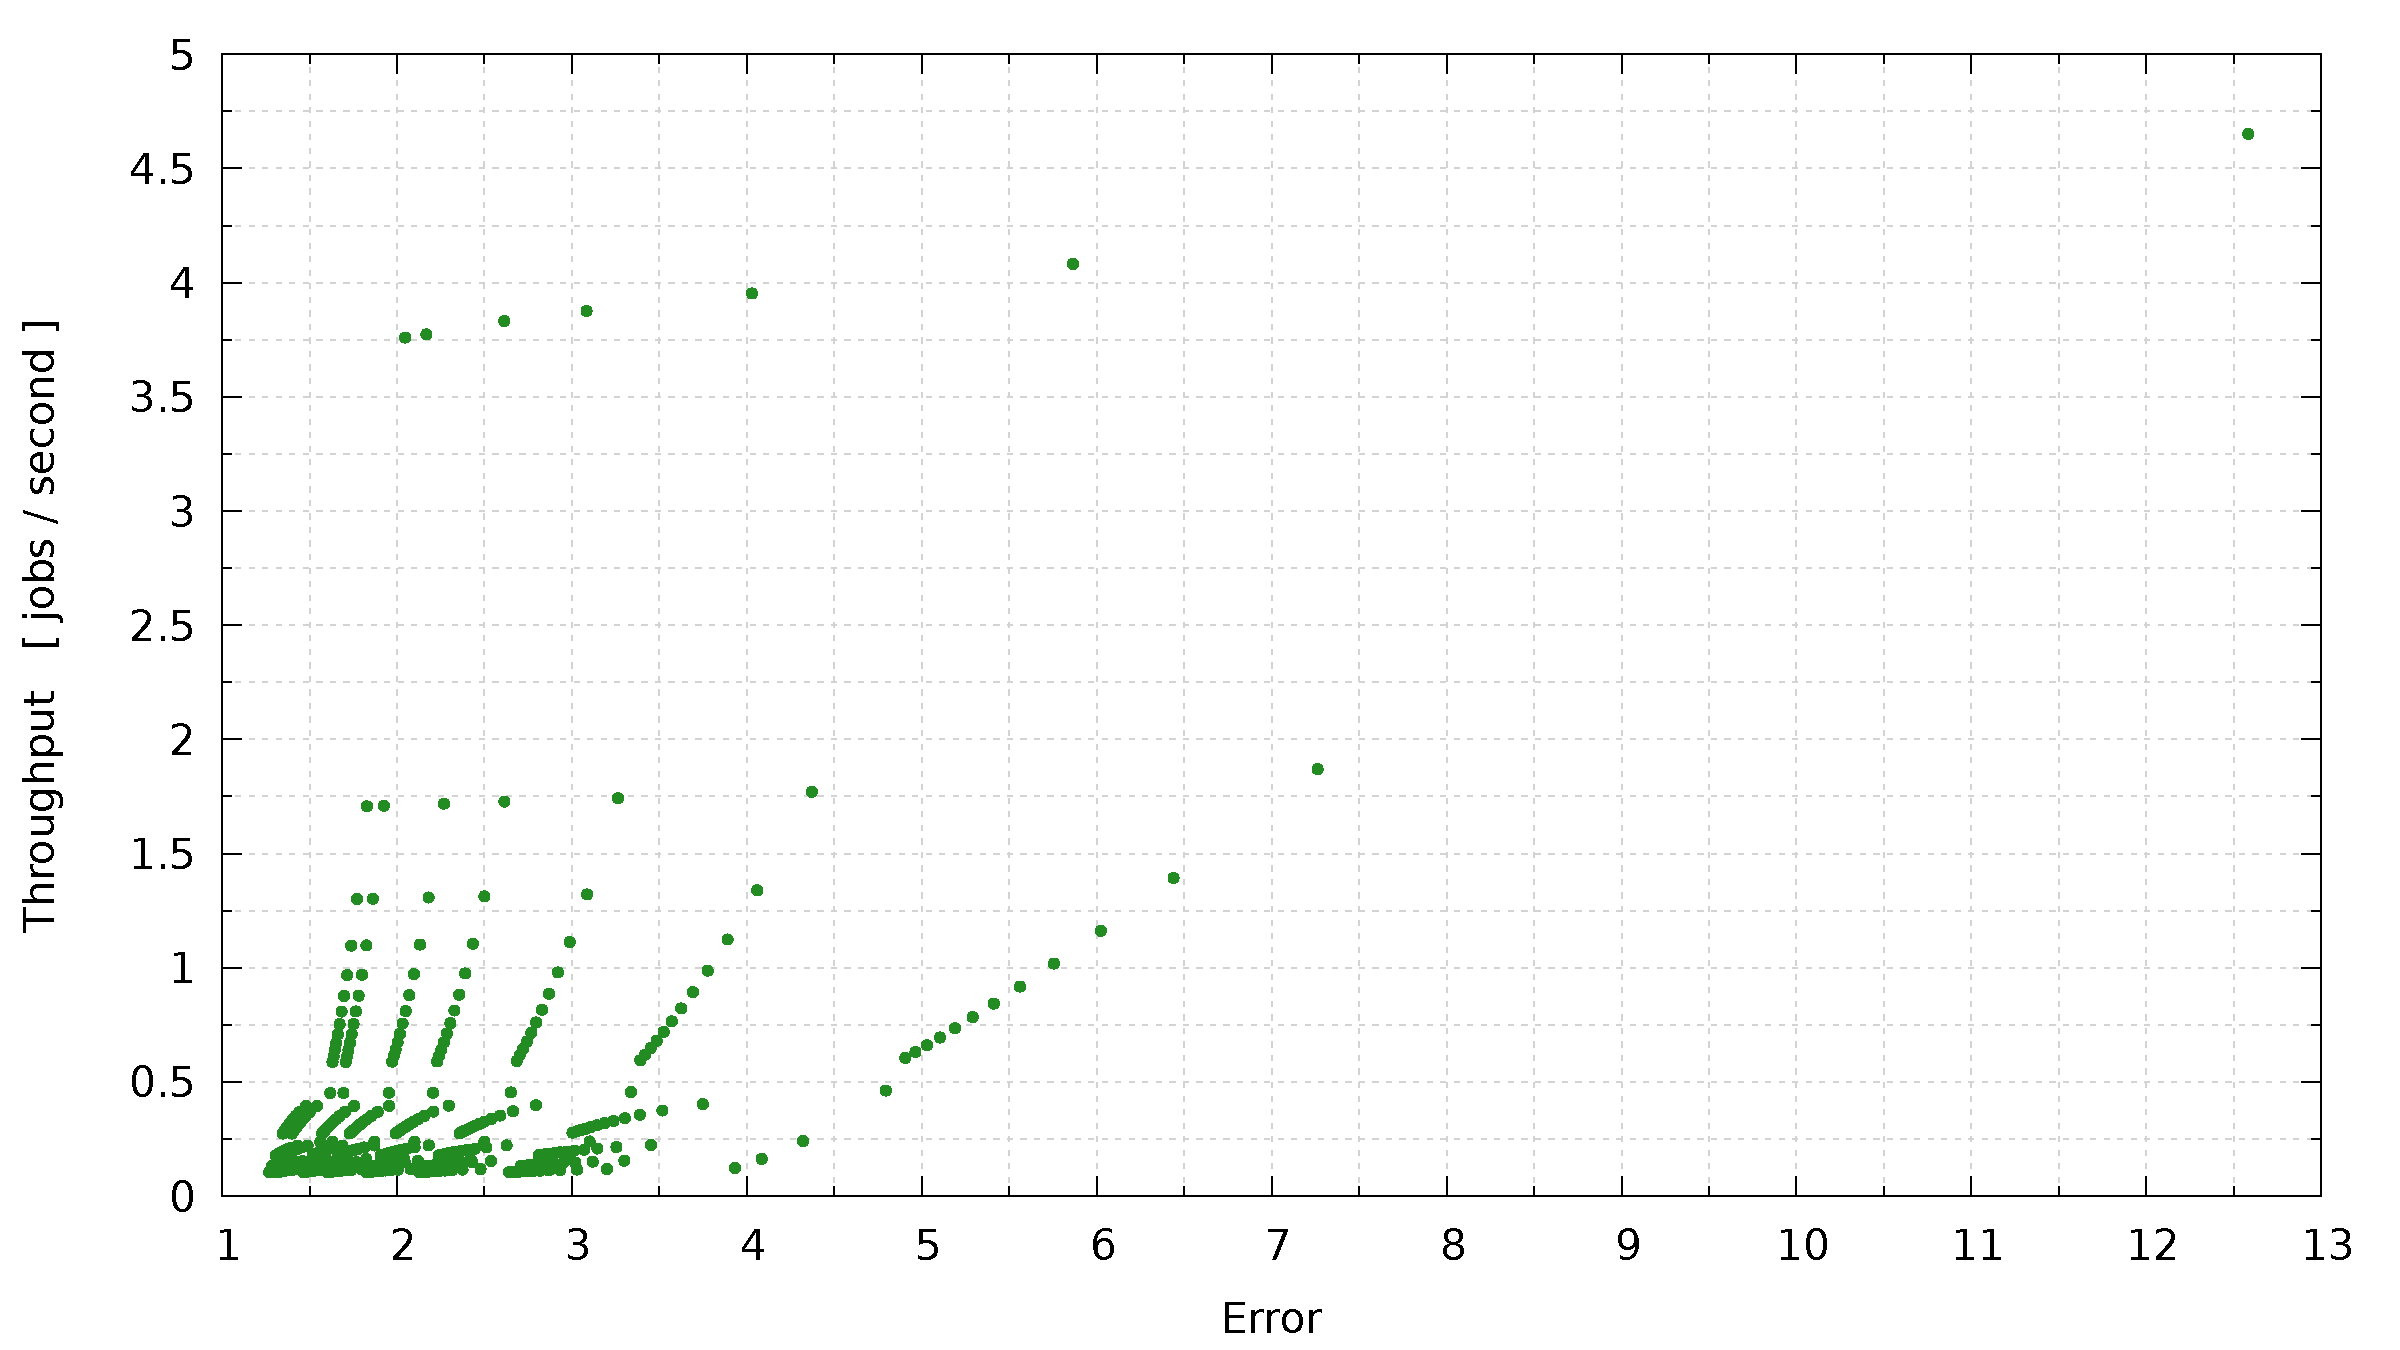
\includegraphics[width = \textwidth]{opGraphSynth1}
    \caption{Throughput by varying the error for synthetic application version 1}
    \label{fig::opListSynth1}
    
\end{figure}

Concerning model prediction quality, therefore, for every application setting with a fixed $noisePercentage$, estimated OP list is compared with the corresponding reference one.


\subsection{Synthetic application version 2}

In the second synthetic application version, execution time is equal to:
\[
executionTime = 7.4 \cdot param_1 \cdot param_2 + 2.1 \cdot (param_3)^2 + noise
\]

where $noise$ is simulated as in the previous application version, while the error is:

\[
error = \dfrac{1}{0.01 \cdot param_1 + 0.7 \cdot \ln{(param_2)} + 0.019 \cdot param_3}
\]

Parameter values are:

\begin{table}[h]

    \centering

    \begin{tabular}{ll}
    
        \toprule
        Parameters & Values \\
        \midrule
        $param_1$ & 1, 10, 15, 25, 40, 65, 80 \\
        $param_2$ & 1, 5, 10, 20 \\
        $param_3$ & 10, 13, 16, 19, 22, 25, 28, 31, 34, 37, 40, 43, 46 \\
        \bottomrule 
    
    \end{tabular}

    \caption{Synthetic application version 2 parameters and related values}

\end{table}

In this application the number of Operating Points is 364; figure \ref{fig::opListSynth2} shows complete OP distribution of reference model with $noise\-Per\-cent\-age = 5\%$: every point stands for a particular configuration with an associated error value (on x-axis) and a throughput one (on y-axis).

\begin{figure}[h]

    \centering
    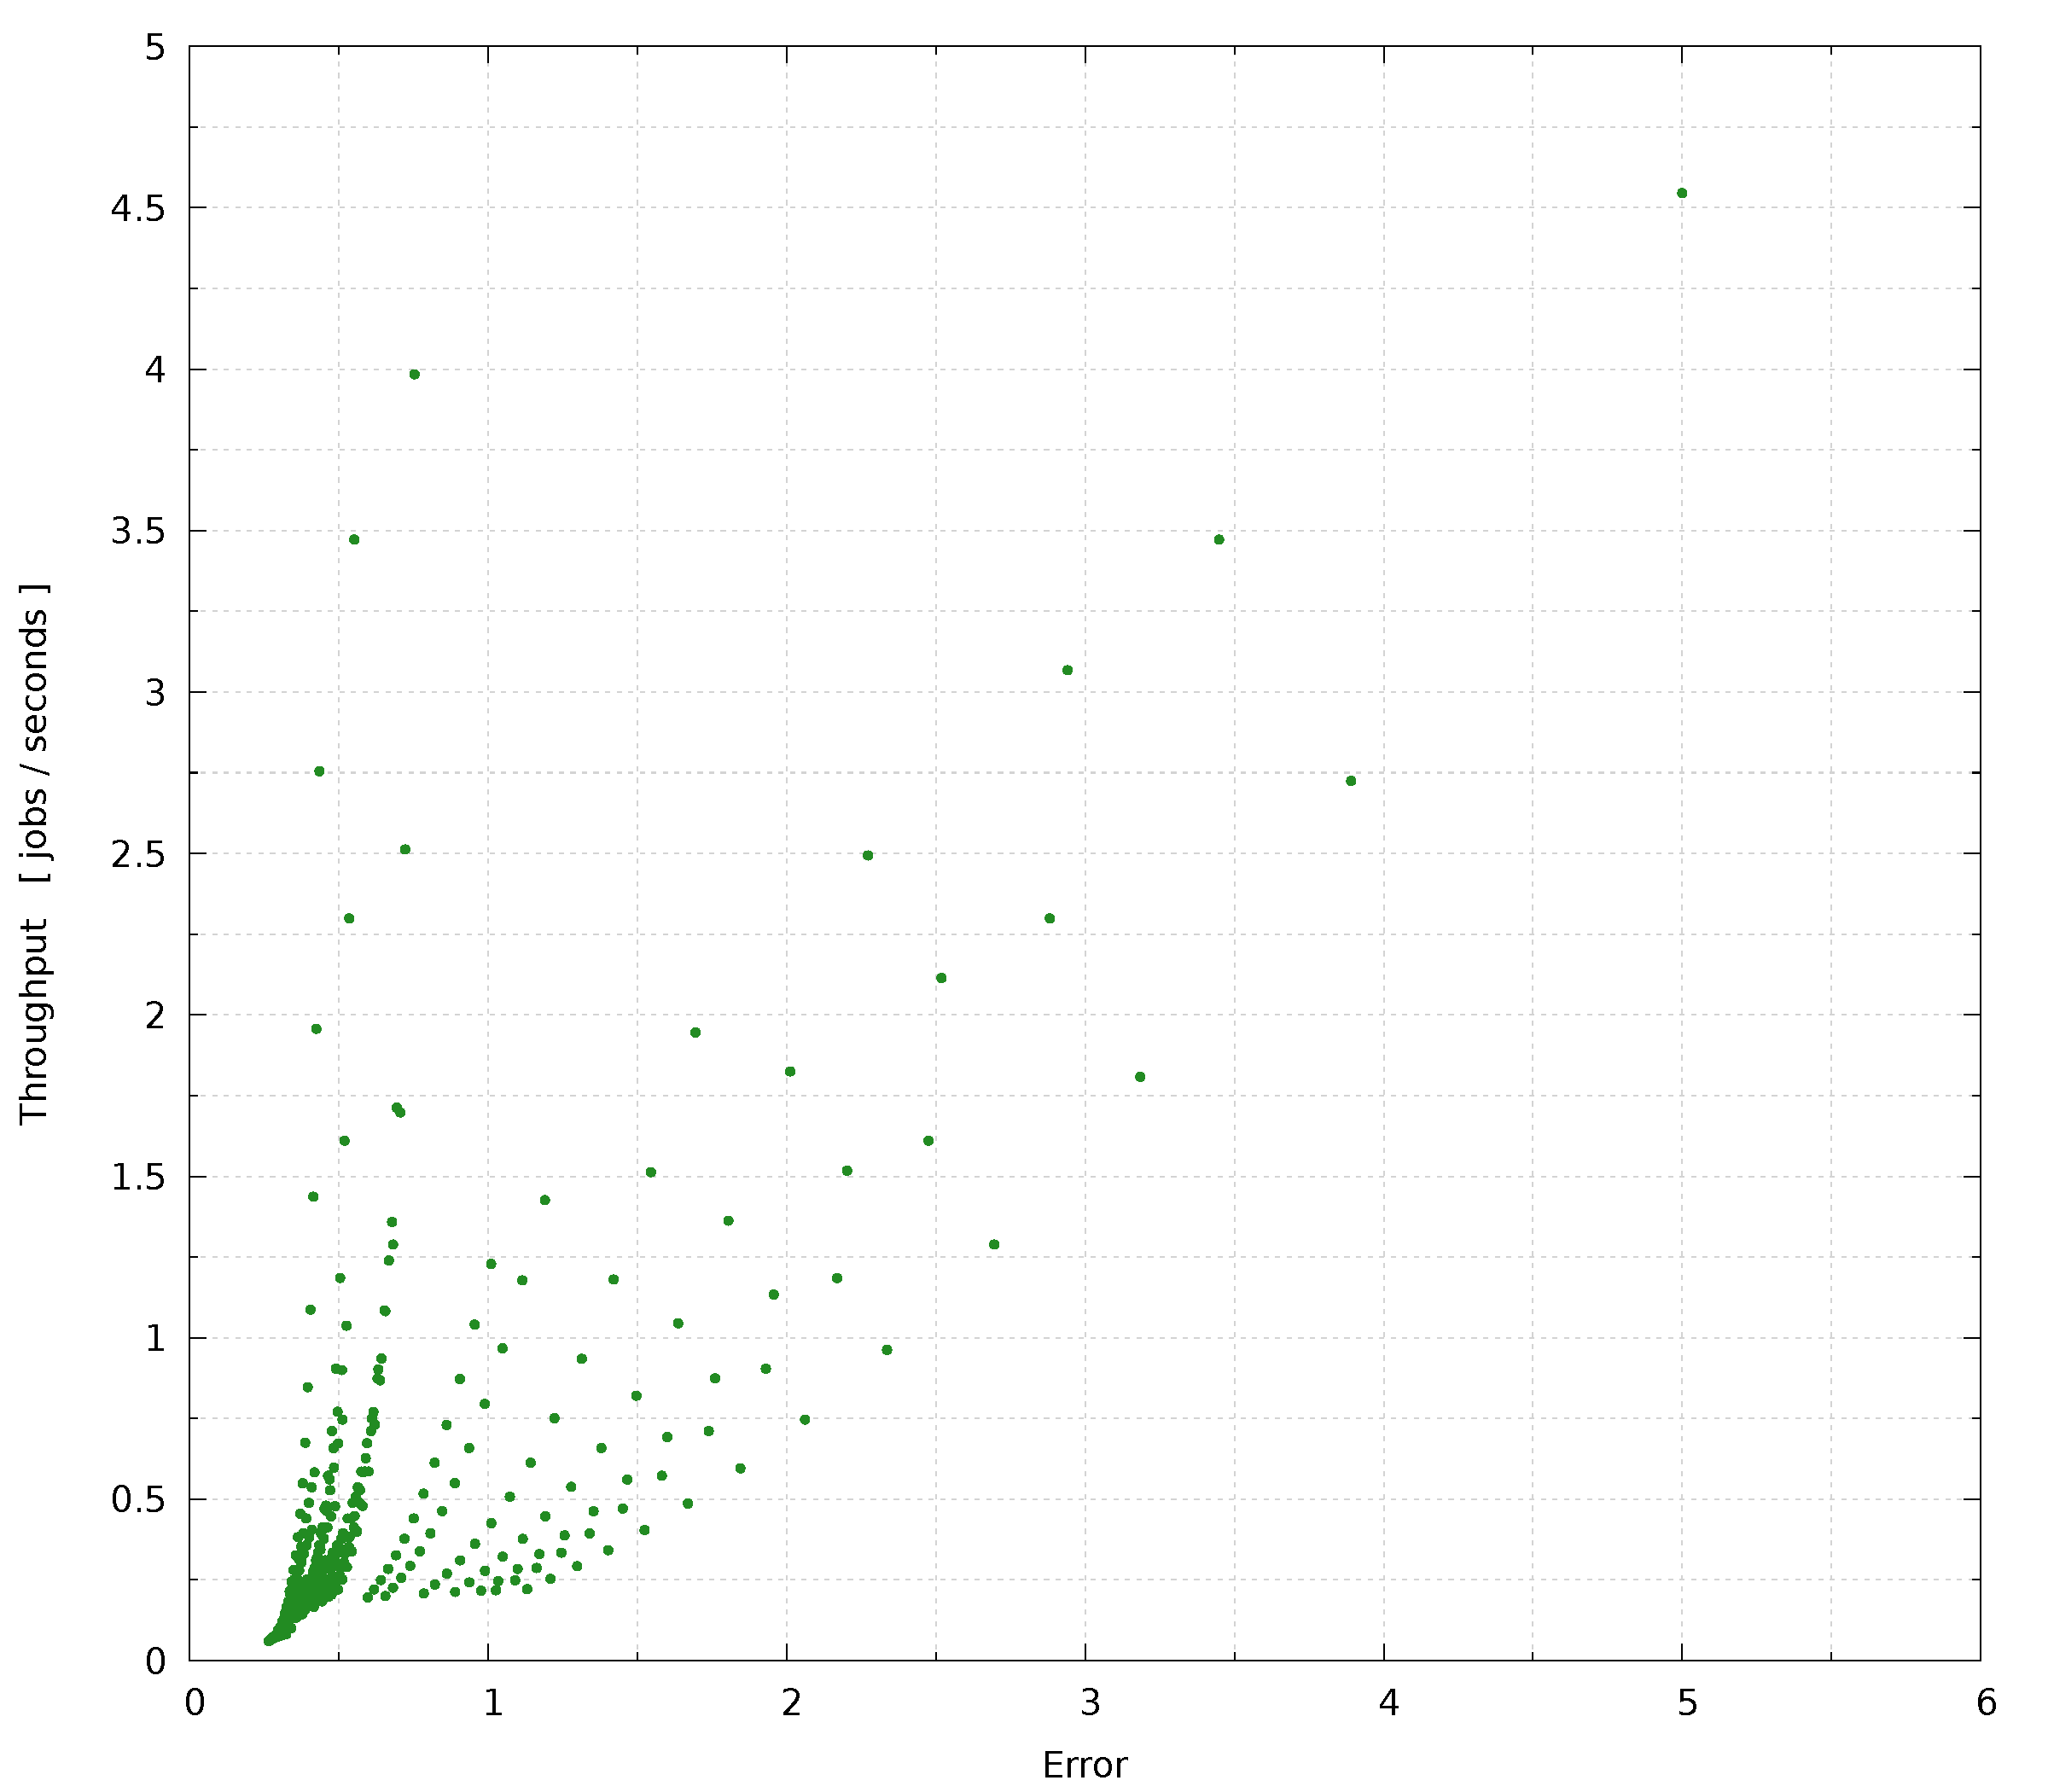
\includegraphics[width = \textwidth]{opGraphSynth2}
    \caption{Throughput by varying the error for synthetic application version 2}
    \label{fig::opListSynth2}
    
\end{figure}

Regarding model prediction goodness, same reasoning as previous application version is applied.


\subsection{Swaptions}

As already stated in \ref{expSetup}, this application has two parameters: $num\_\-threads$ and $num\_\-trials$; their values are:

\begin{table}[h]

    \centering

    \begin{tabular}{ll}
    
        \toprule
        Parameters & Values \\
        \midrule
        $num\_threads$ & 1, 2, 3, 4, 5, 6, 7, 8 \\
        $num\_trials (\cdot 10^3)$ & 100, 200, 300, 400, 500, 600, 700, 800, 900, 1000 \\
        \bottomrule 
    
    \end{tabular}

    \caption{Swaptions parameters and related values}

\end{table}

The number of Operating Points is therefore 80; figure \ref{fig::swaptionsOPs} shows complete OP distribution with respect $avg\_error$ and $avg\_throughput$ metrics of interest:

\begin{figure}[h]

    \centering
    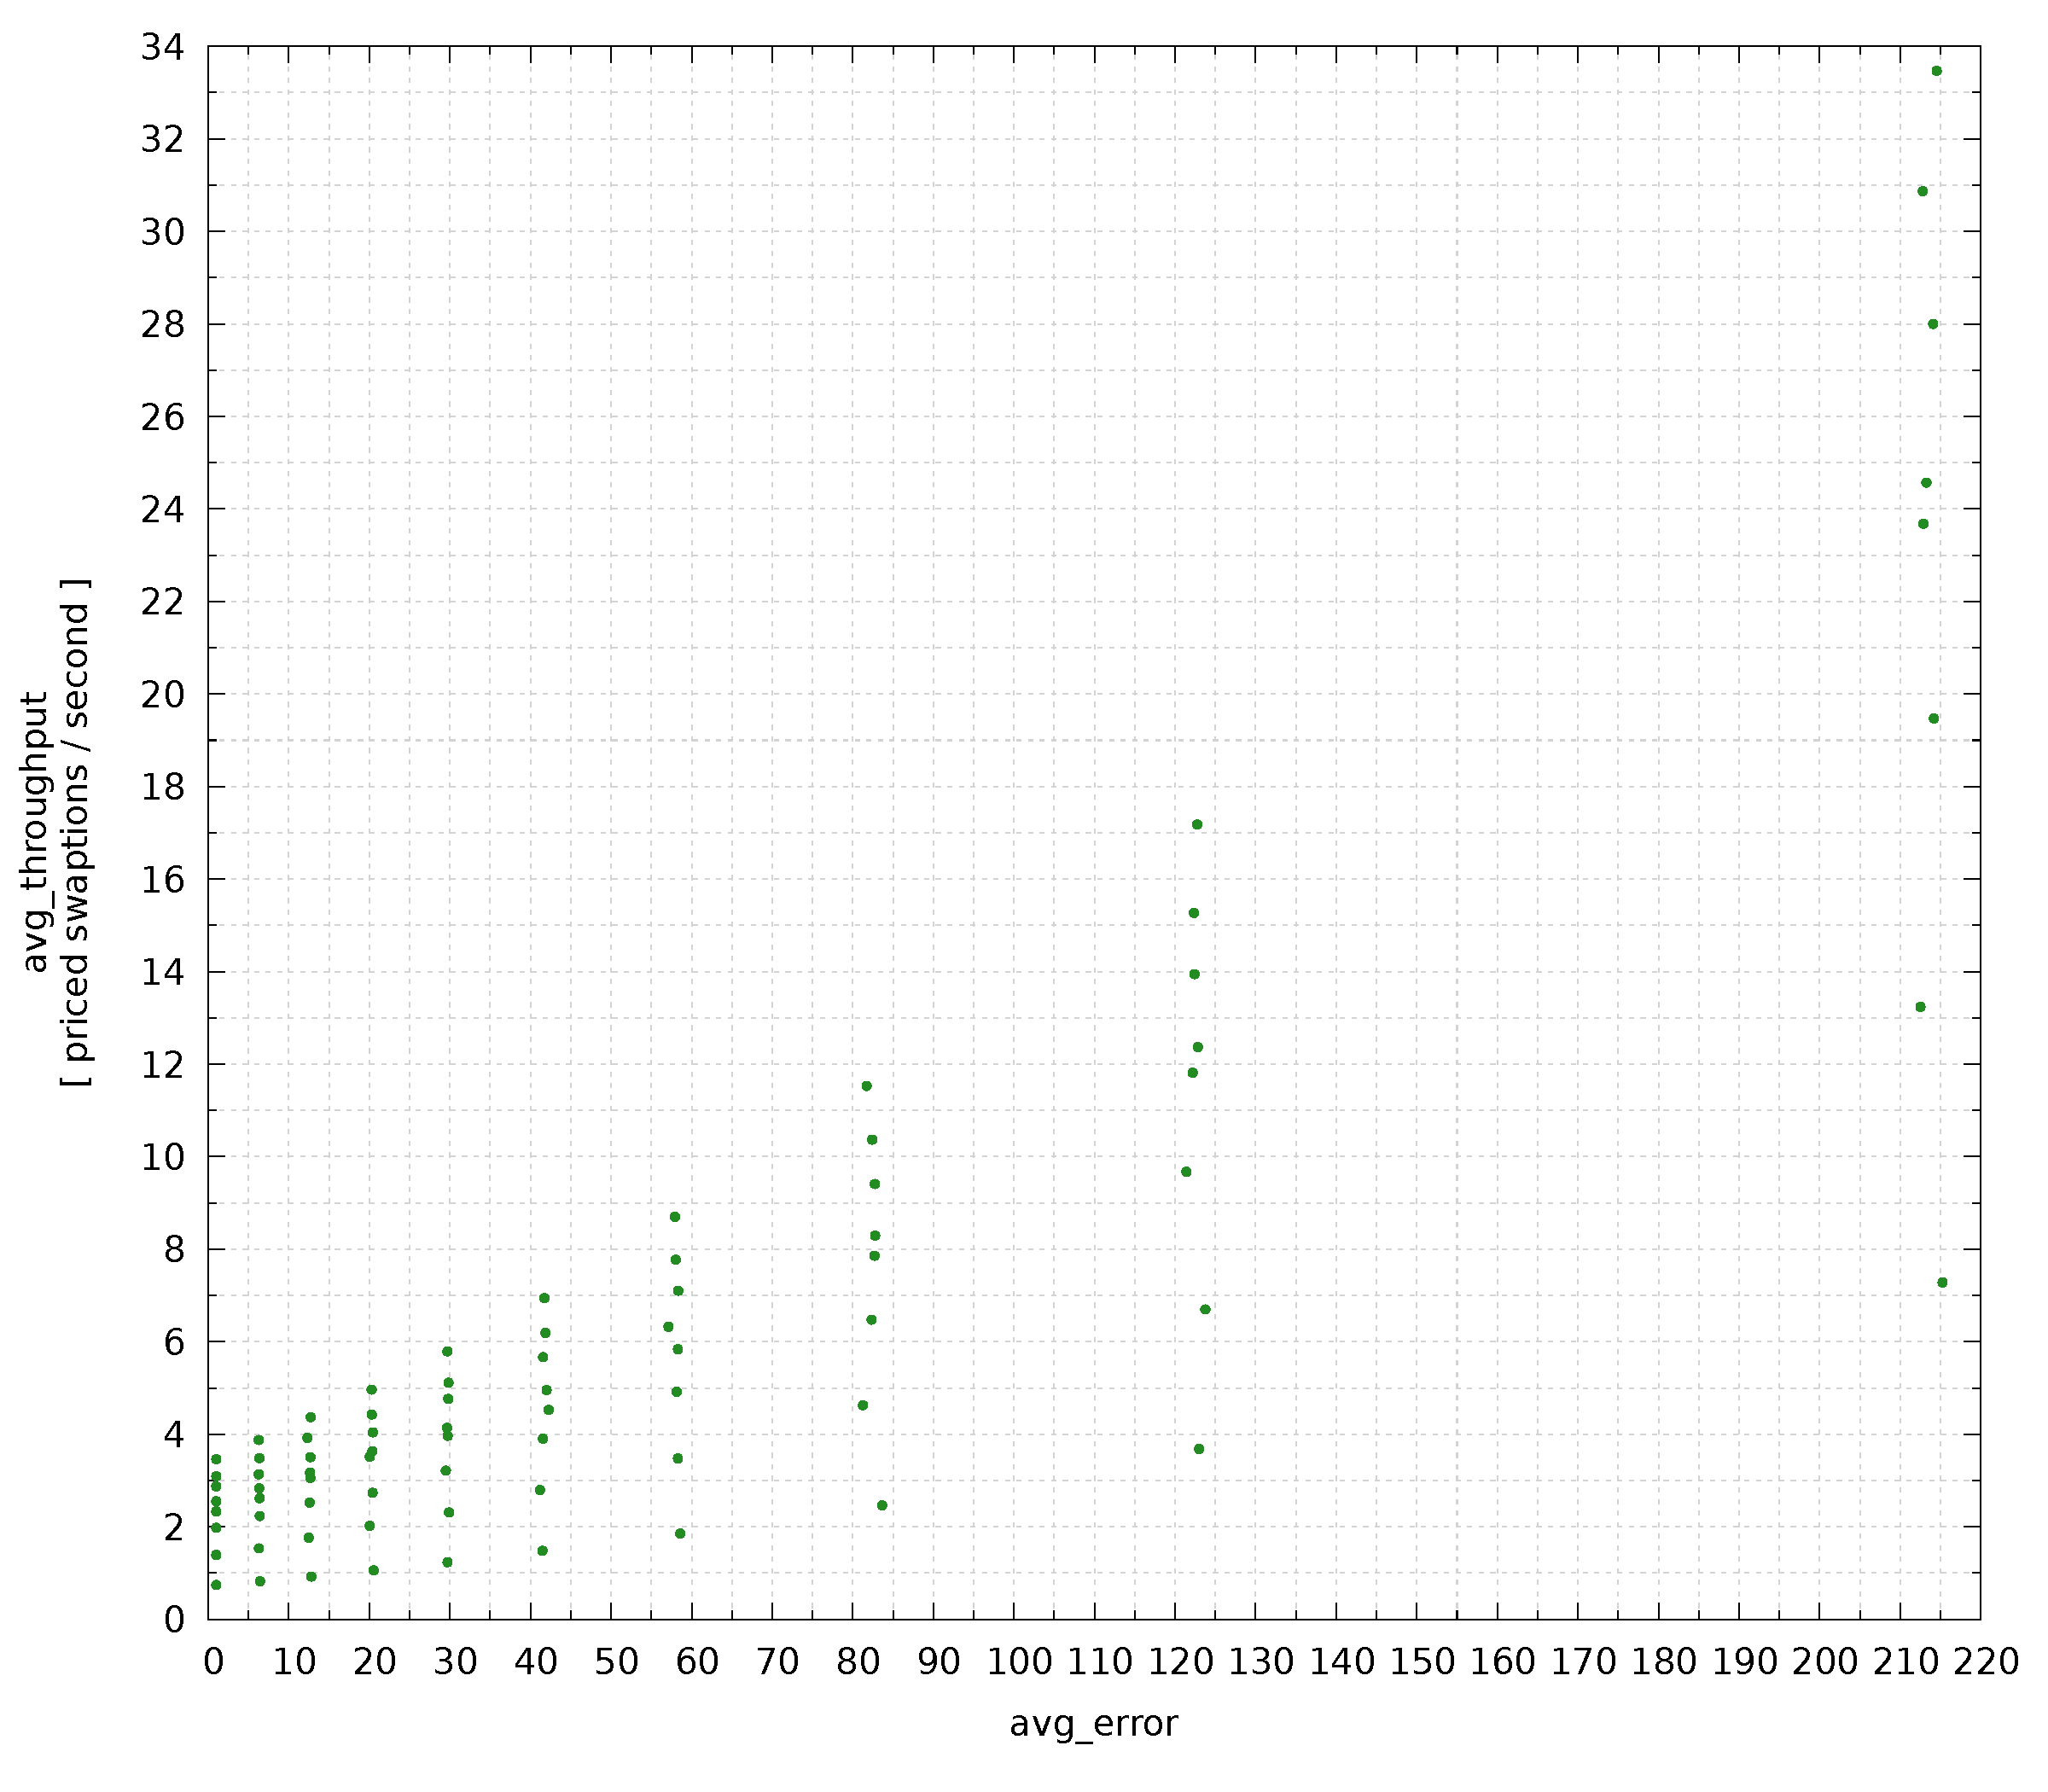
\includegraphics[width = \textwidth]{swaptionsOPgraph}
    \caption{Average throughput by varying the average error for Swaptions}
    \label{fig::swaptionsOPs}
    
\end{figure}





\section{Experimental campaign}\label{campaign}

We want to demonstrate Agorà validity; for both synthetic application versions and \textit{Swaptions}, we focuse our attention on model prediction goodness in various scenarios; we study execution times, especially for Design Space Exploration phases with one and more than one executing applications at the same time, highlighting benefits in sharing DSE; we reveal application behavior during execution on different cases; next paragraphs show results, firstly for synthetic applications, finally for the real one.


\subsection{Synthetic application}

In this paragraph we show experimental results for both versions of synthetic application, divided as explained before.


\subsubsection{Model prediction quality}\label{deltaErrorExplanation}

Concerning model prediction goodness, both synthetic application versions are executed several times with the introduction of all noise weights ($1\%, 5\%, 10\%, 15\%, 25\%$ and $50\%$), focusing on the prediction of throughput metric, that is the one affected by $noise\-Percentage$ value; a Face Centered Central Composite Desing of Experiments with one Center Point has been used, firstly gathering 1 repetition, then 5 repetitions and finally 10 repetitions for each DoE configuration during Design Space Exploration phase; for each predicted metric value $m$ for each application setting, we have calculated a $deltaError$ measure:

\[
deltaError(m) = \dfrac{\left\vert predictedValue(m) - referenceValue(m) \right\vert \cdot 100}{\left\vert referenceValue(m) \right\vert}
\]

where $predictedValue(m)$ and $referenceValue(m)$ have explicit meaning; so, $deltaError(m)$ stands for how much the predicted metric value $m$ distances itself from the corresponding value of the related reference model, in percentage; next figures summarize results:





\begin{figure}[h]

    \centering
    
    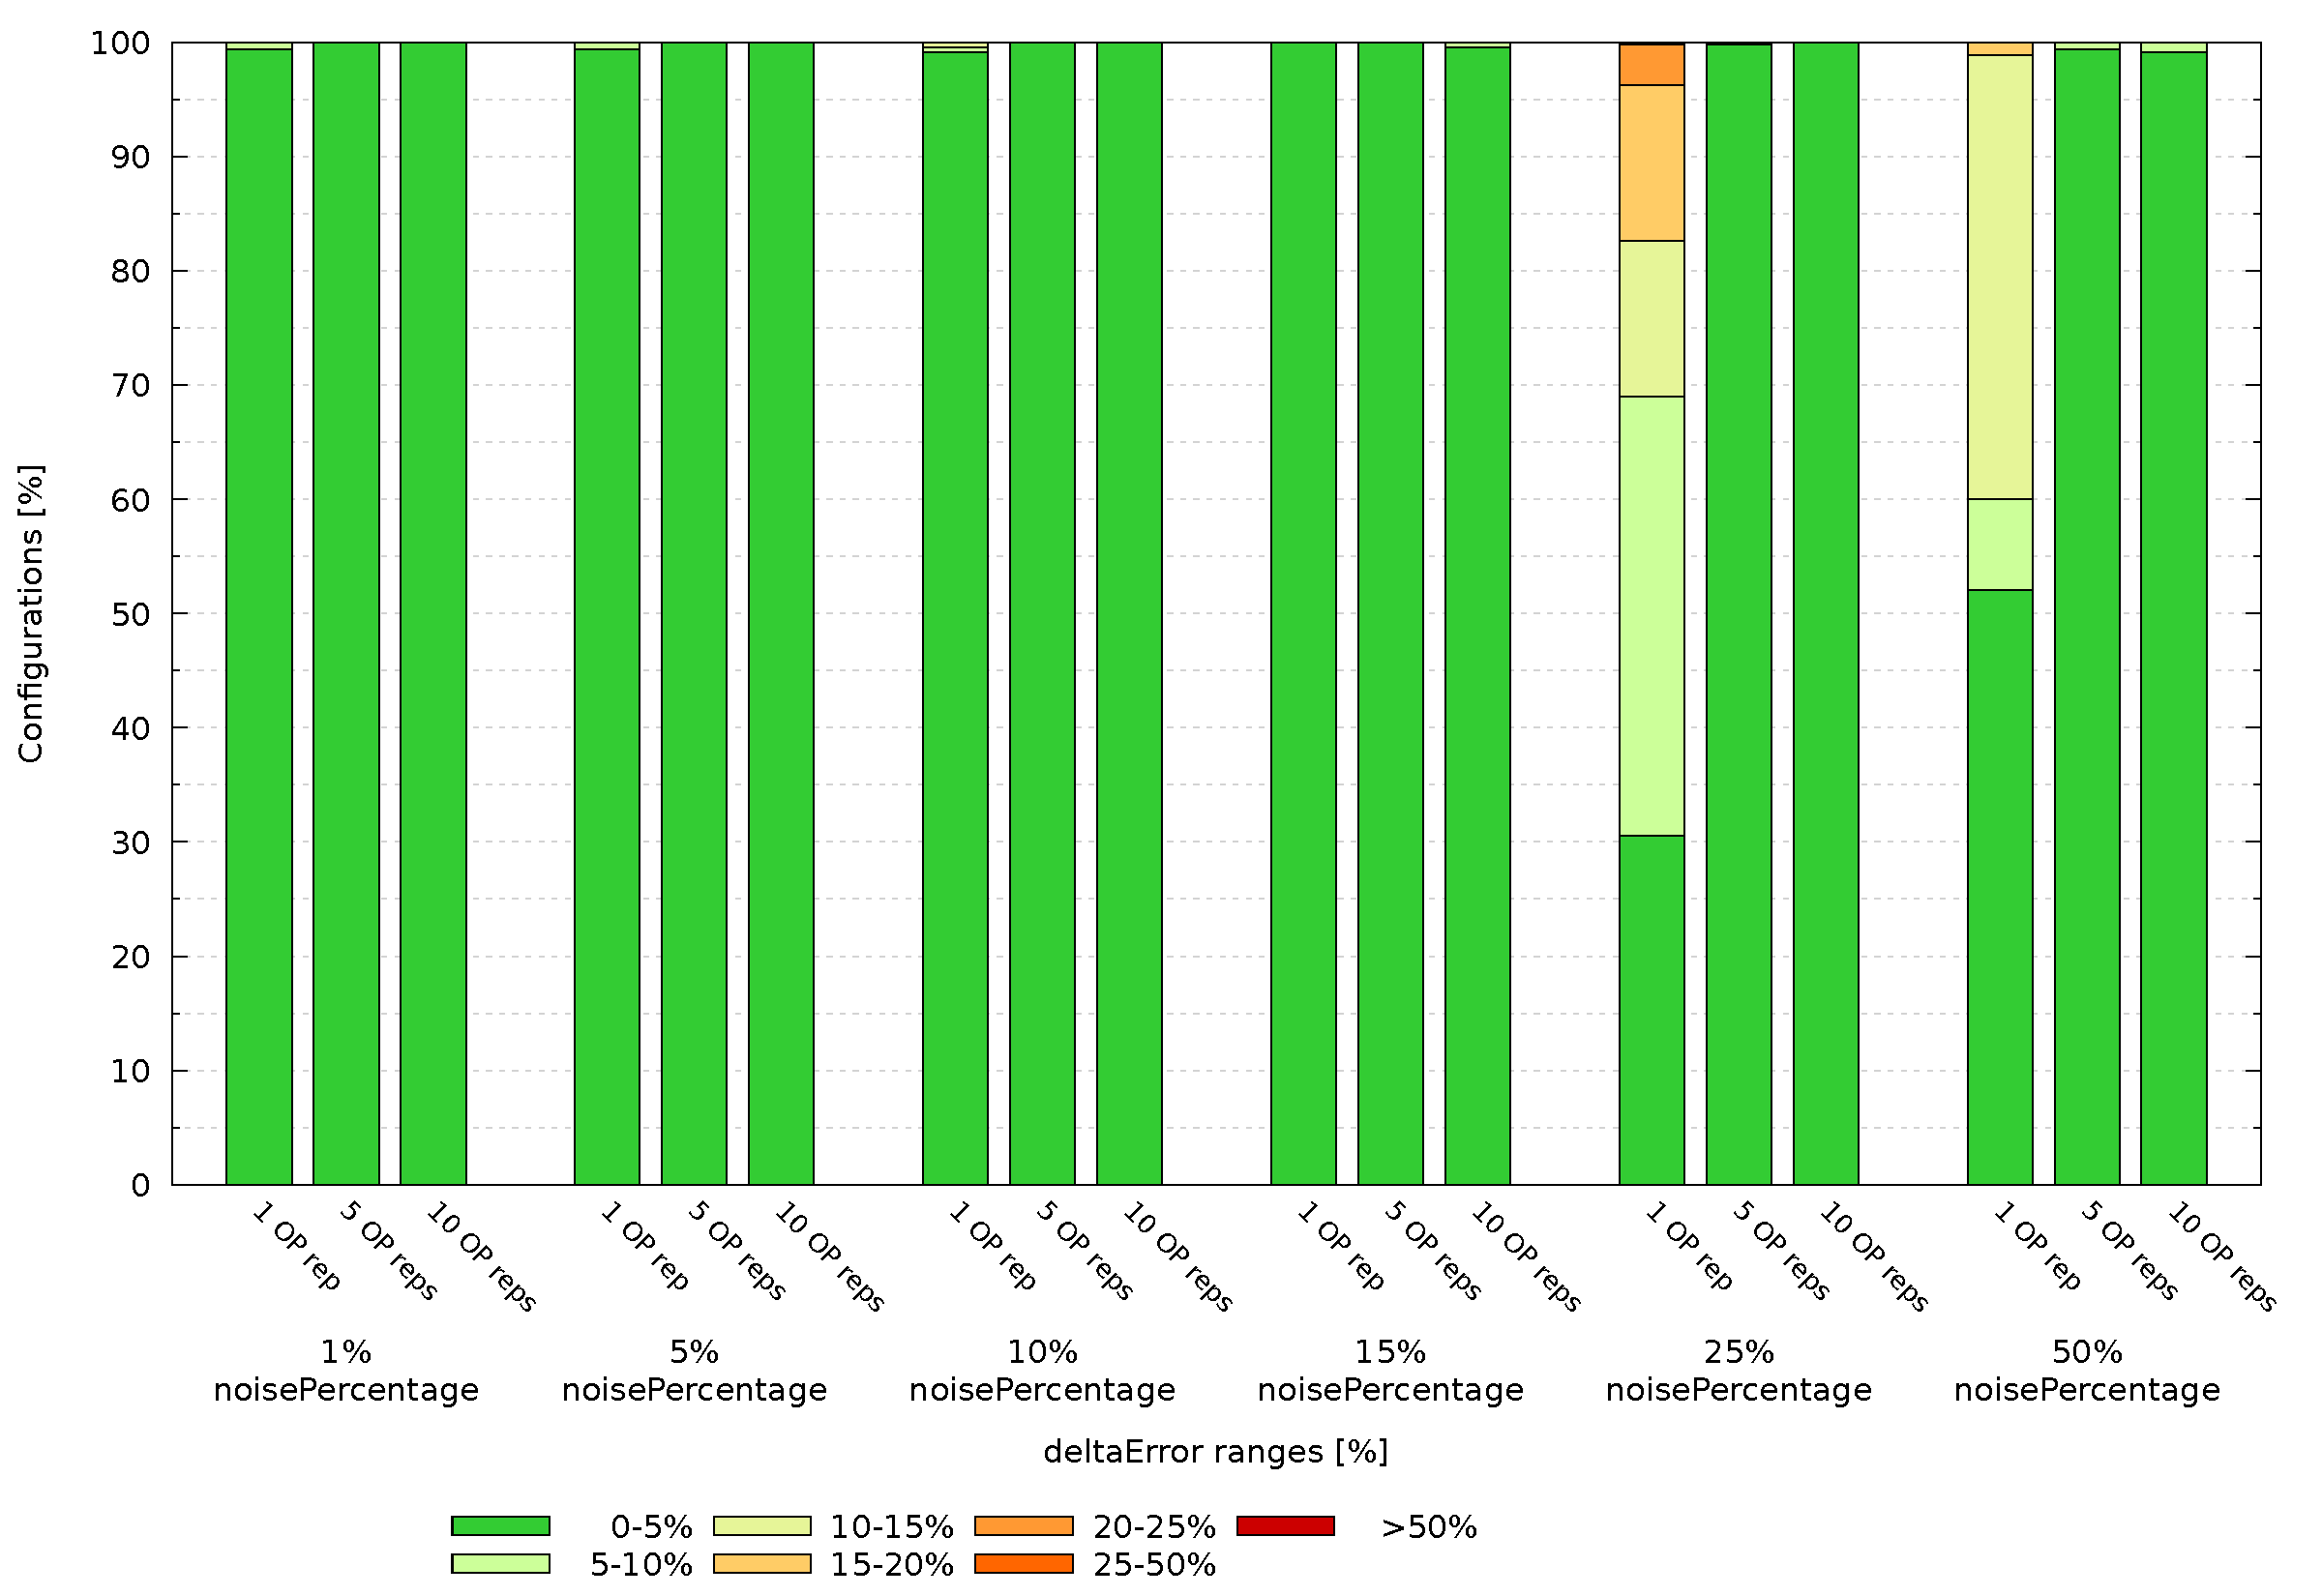
\includegraphics[width = \textwidth]{deltaErrorRangesSynth1spark1}
    
     \caption{$deltaError$ results for throughput metric of synthetic application version 1 by varying the noisePercentage and the number of OP repetitions. Used RSM: 1st version of implemented GLR ("transformations by functions")}
    
    \label{fig::synth1spark1::intervals}
    
\end{figure}

\begin{figure}[h]

    \centering
    
    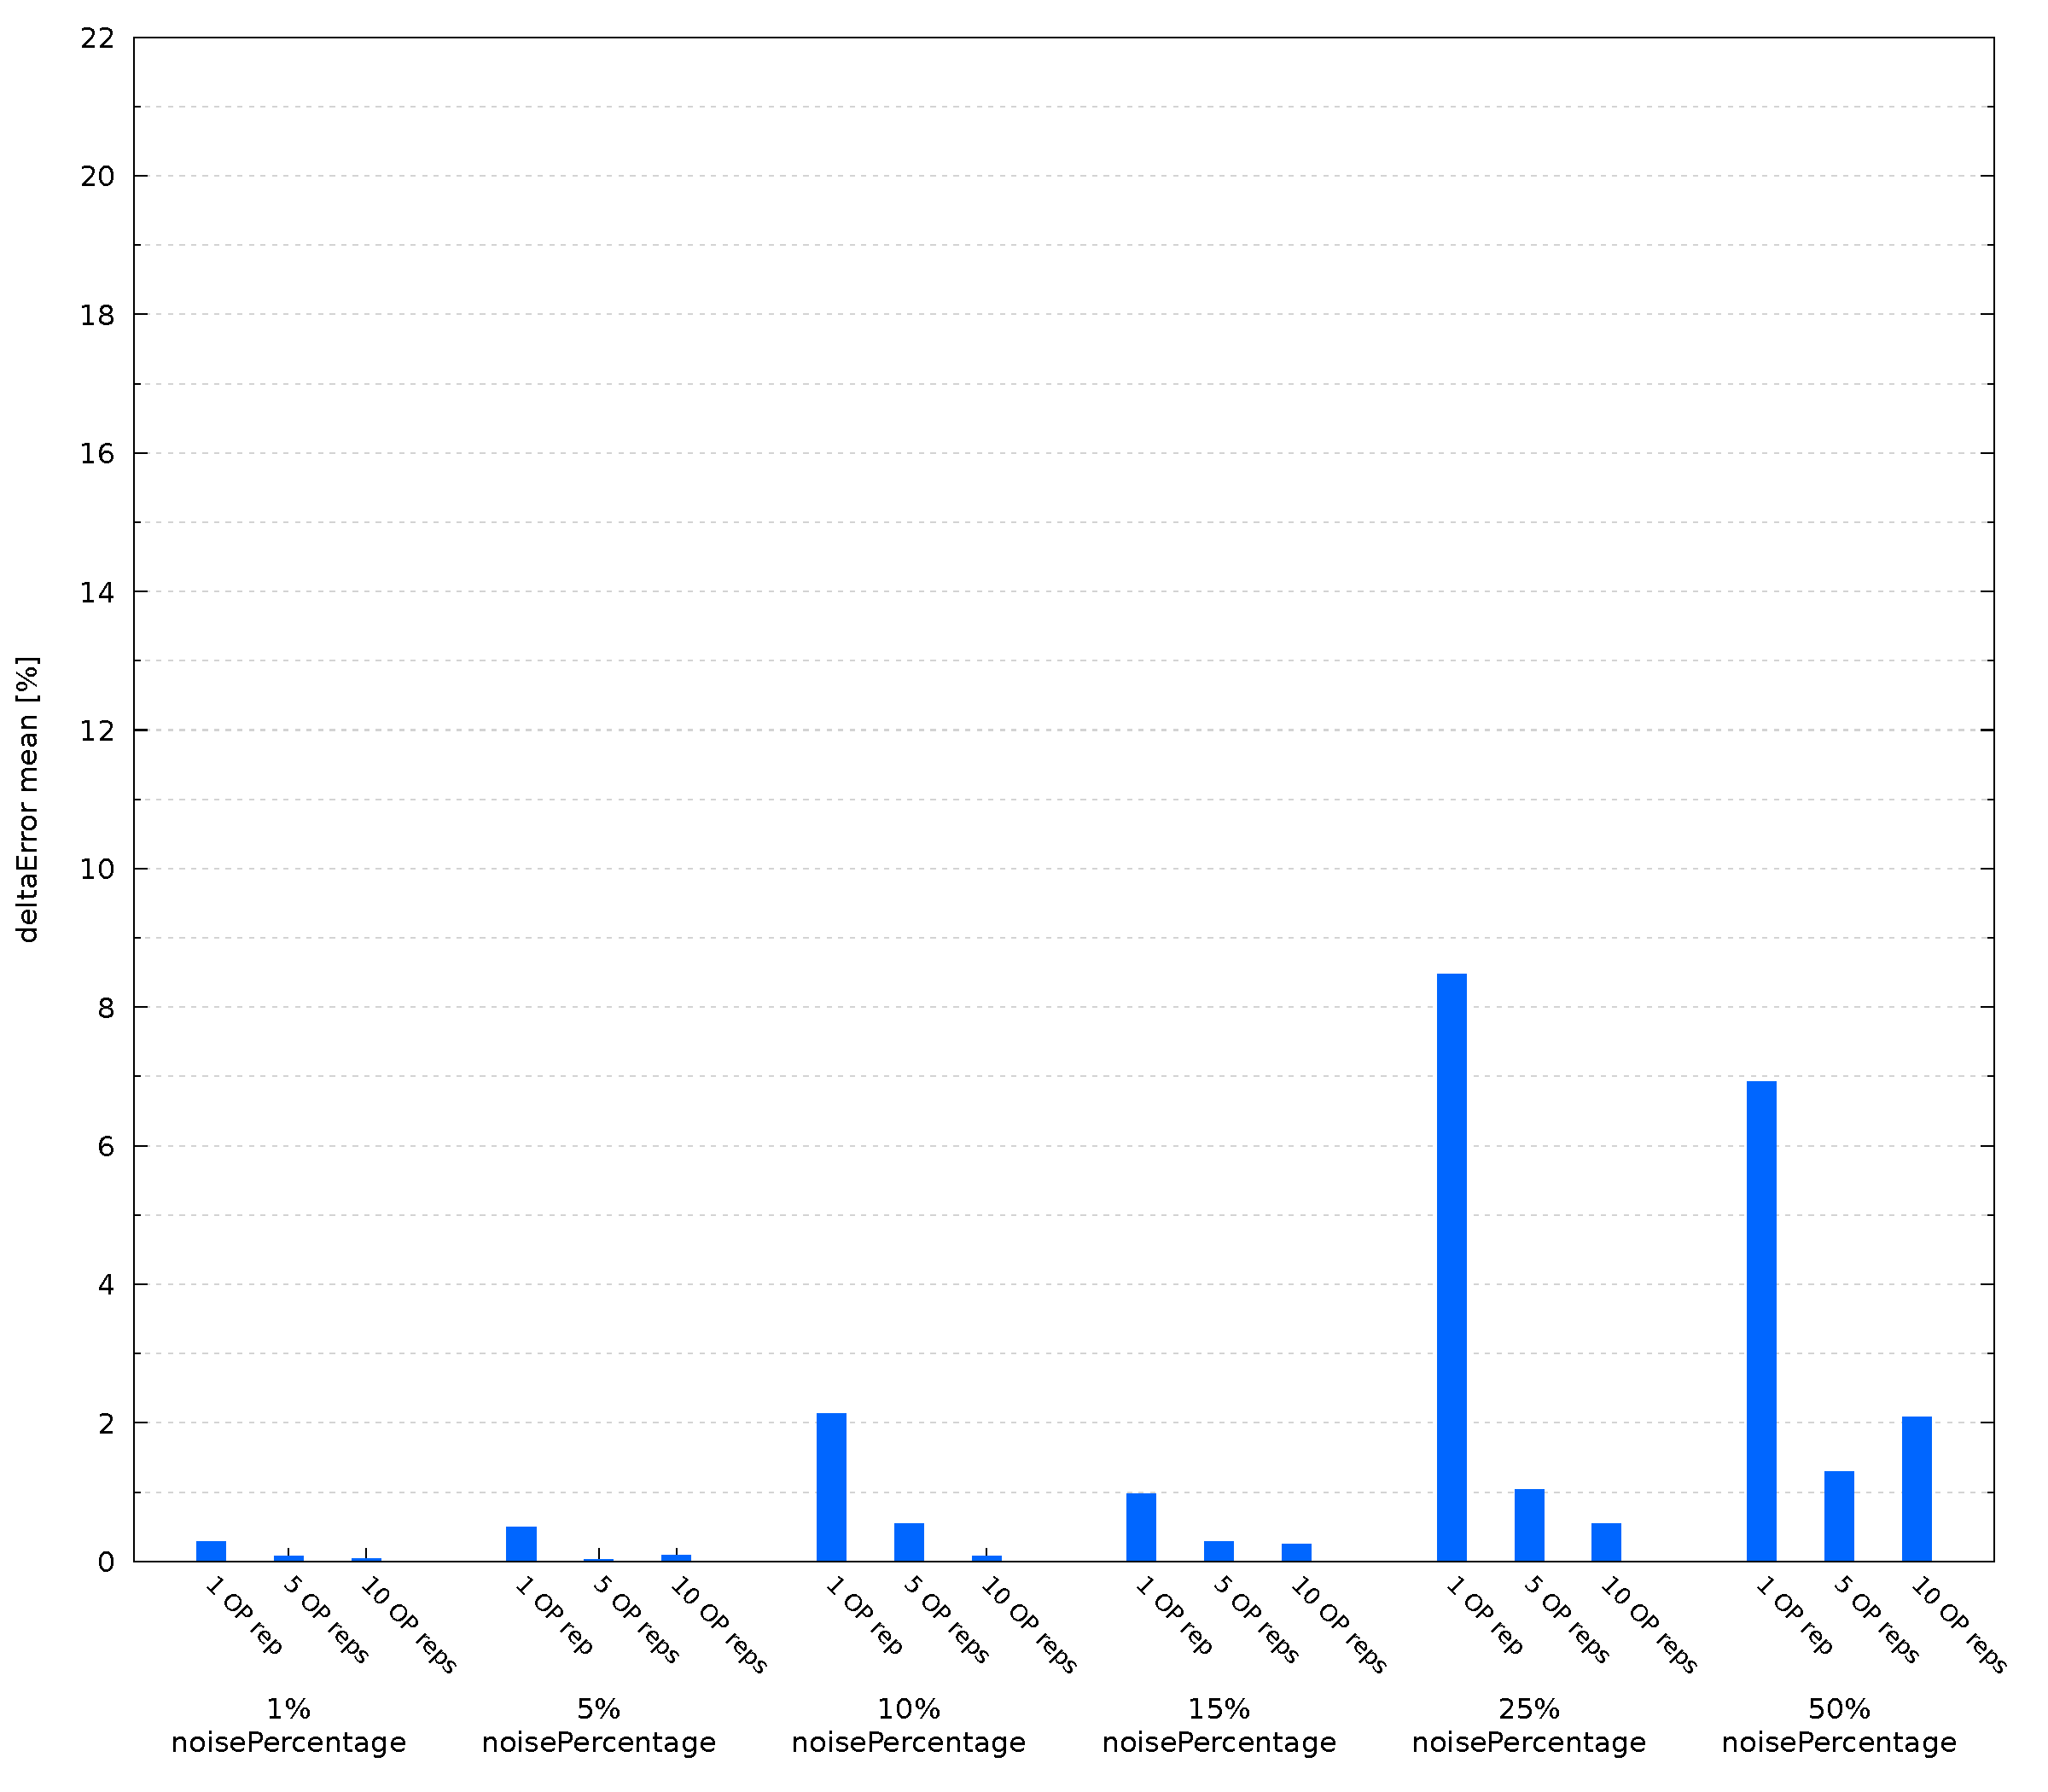
\includegraphics[width = \textwidth]{deltaErrorMeansSynth1spark1}
    
    \caption{$deltaError$ mean for throughput metric of synthetic application version 1 by varying the noisePercentage and the number of OP repetitions. Used RSM: 1st version of implemented GLR ("transformations by functions")}
    
    \label{fig::synth1spark1::means}
    
\end{figure}





\begin{figure}[h]

    \centering
    
    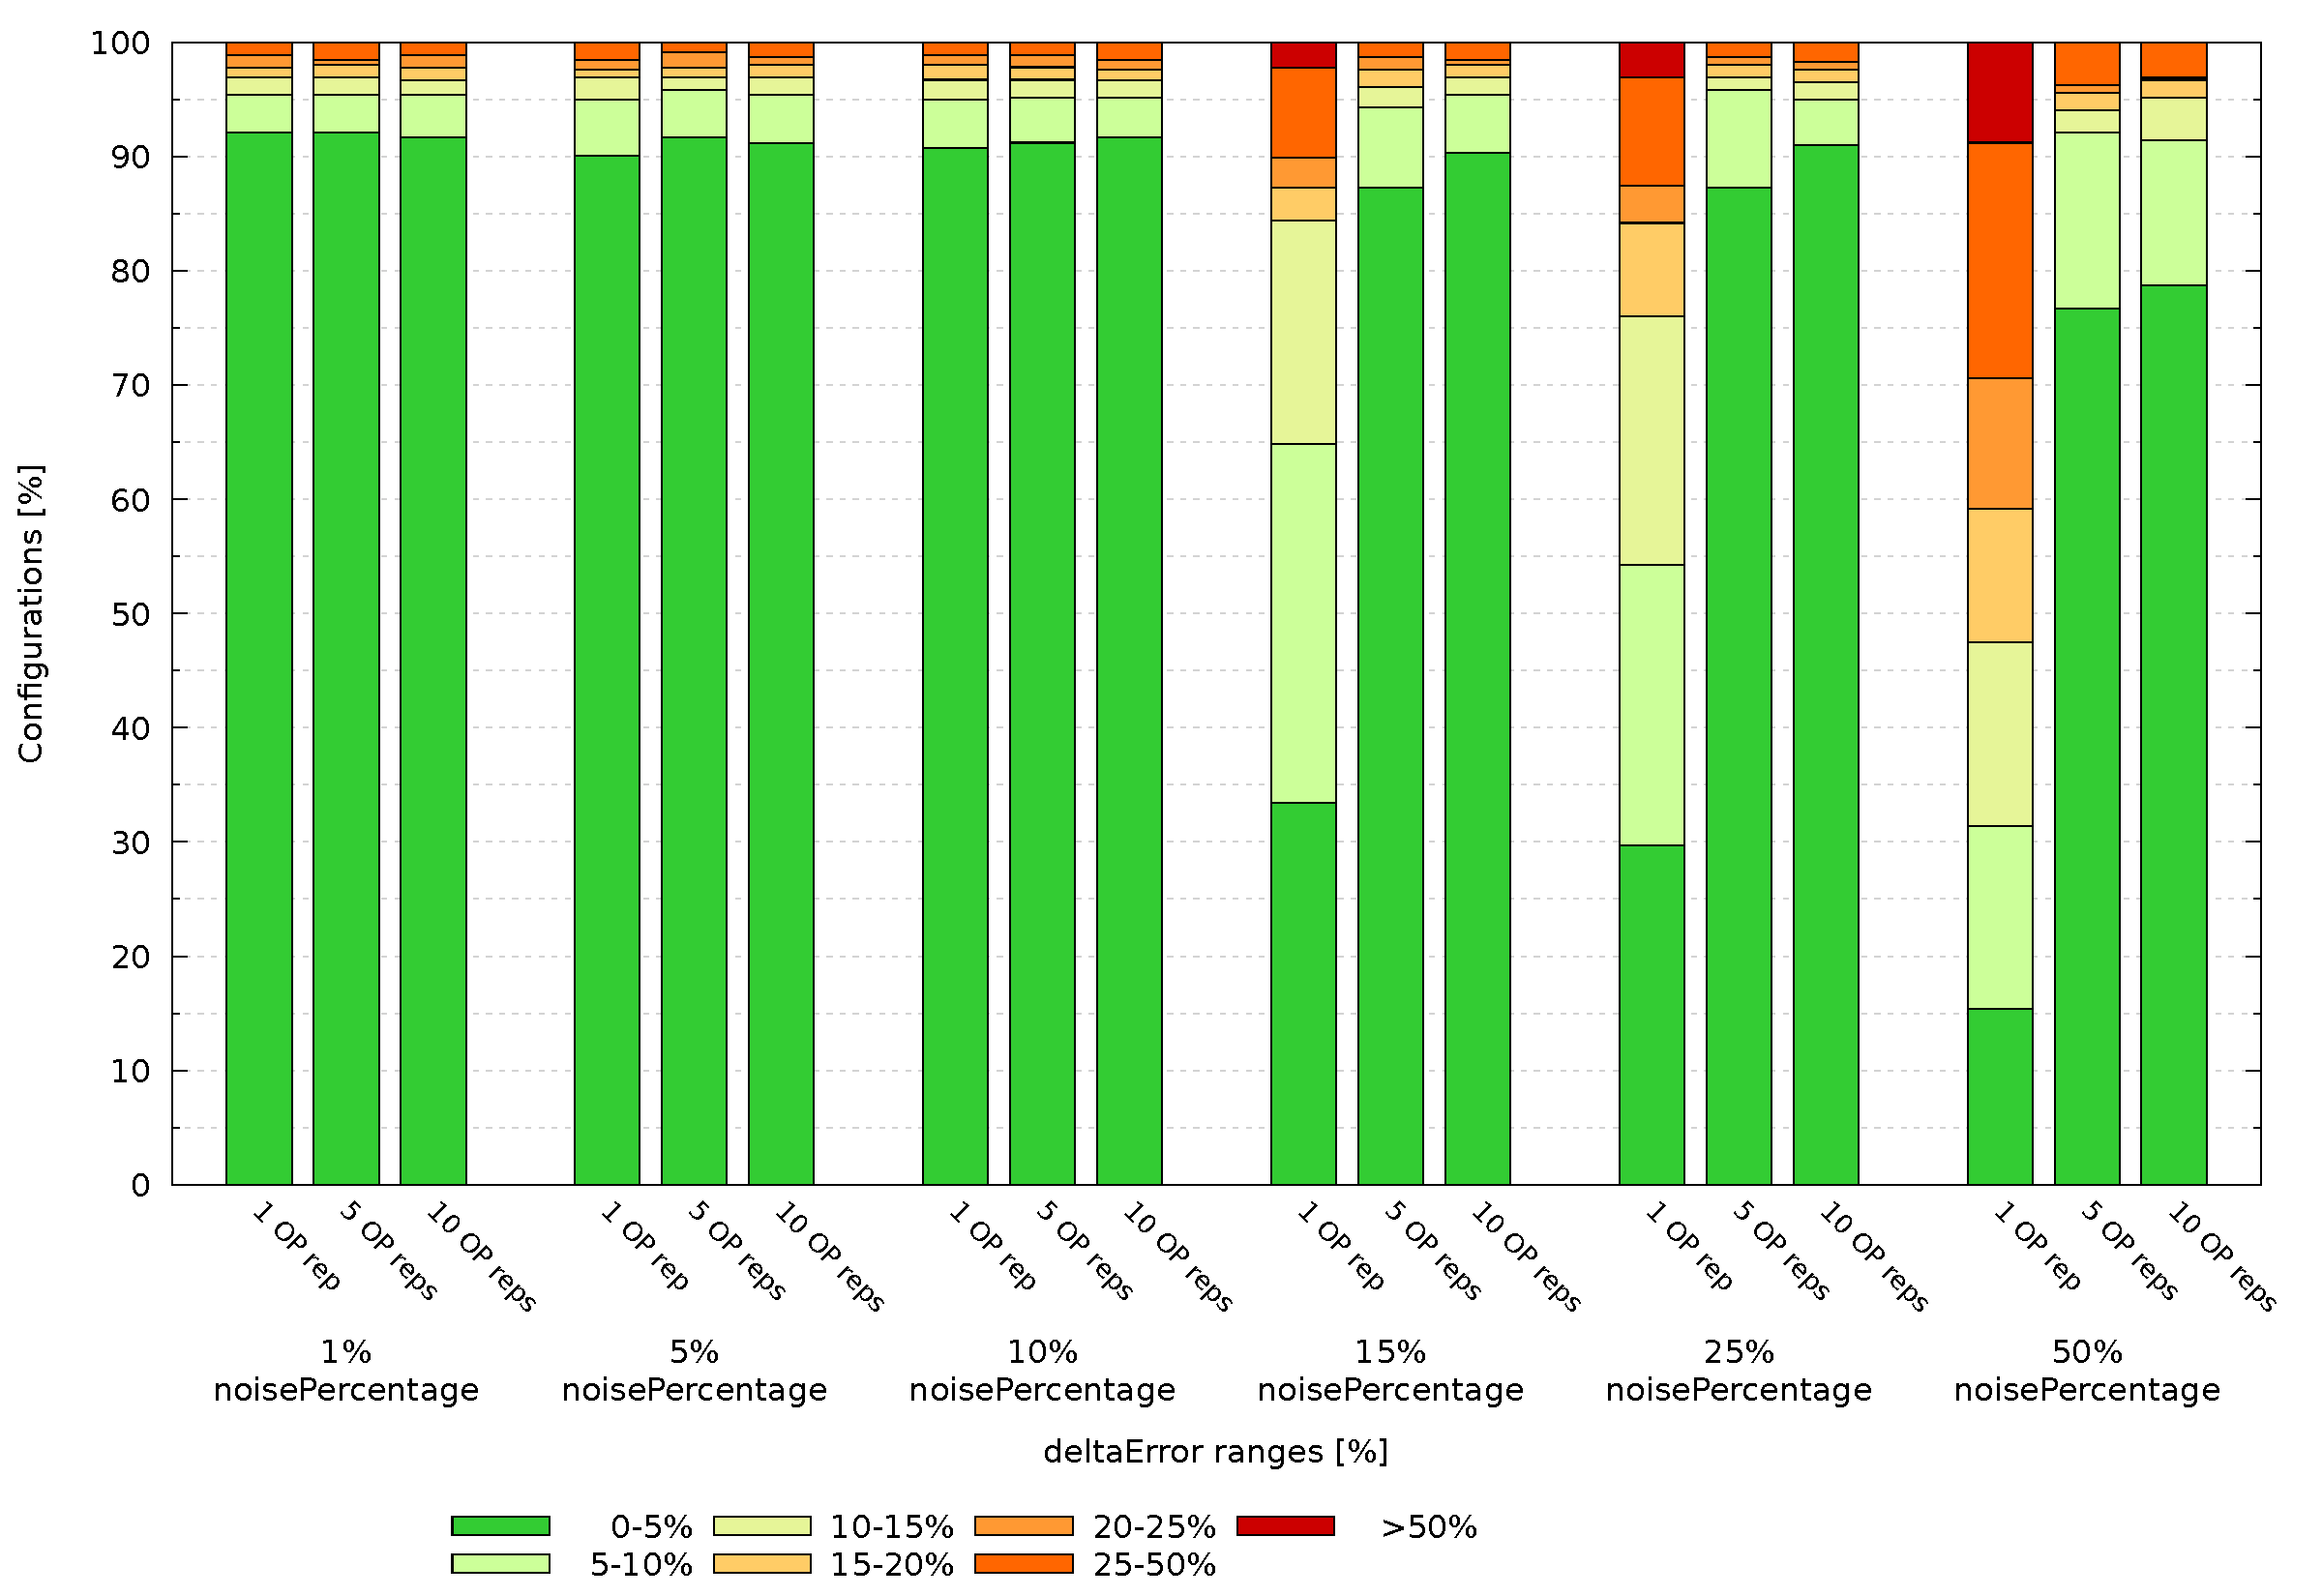
\includegraphics[width = \textwidth]{deltaErrorRangesSynth1spark2}
    
     \caption{$deltaError$ results for throughput metric of synthetic application version 1 by varying the noisePercentage and the number of OP repetitions. Used RSM: 2nd version of implemented GLR ("polynomial combinations of degree 2")}
    
    \label{fig::synth1spark2::intervals}
    
\end{figure}

\begin{figure}[h]

    \centering
    
    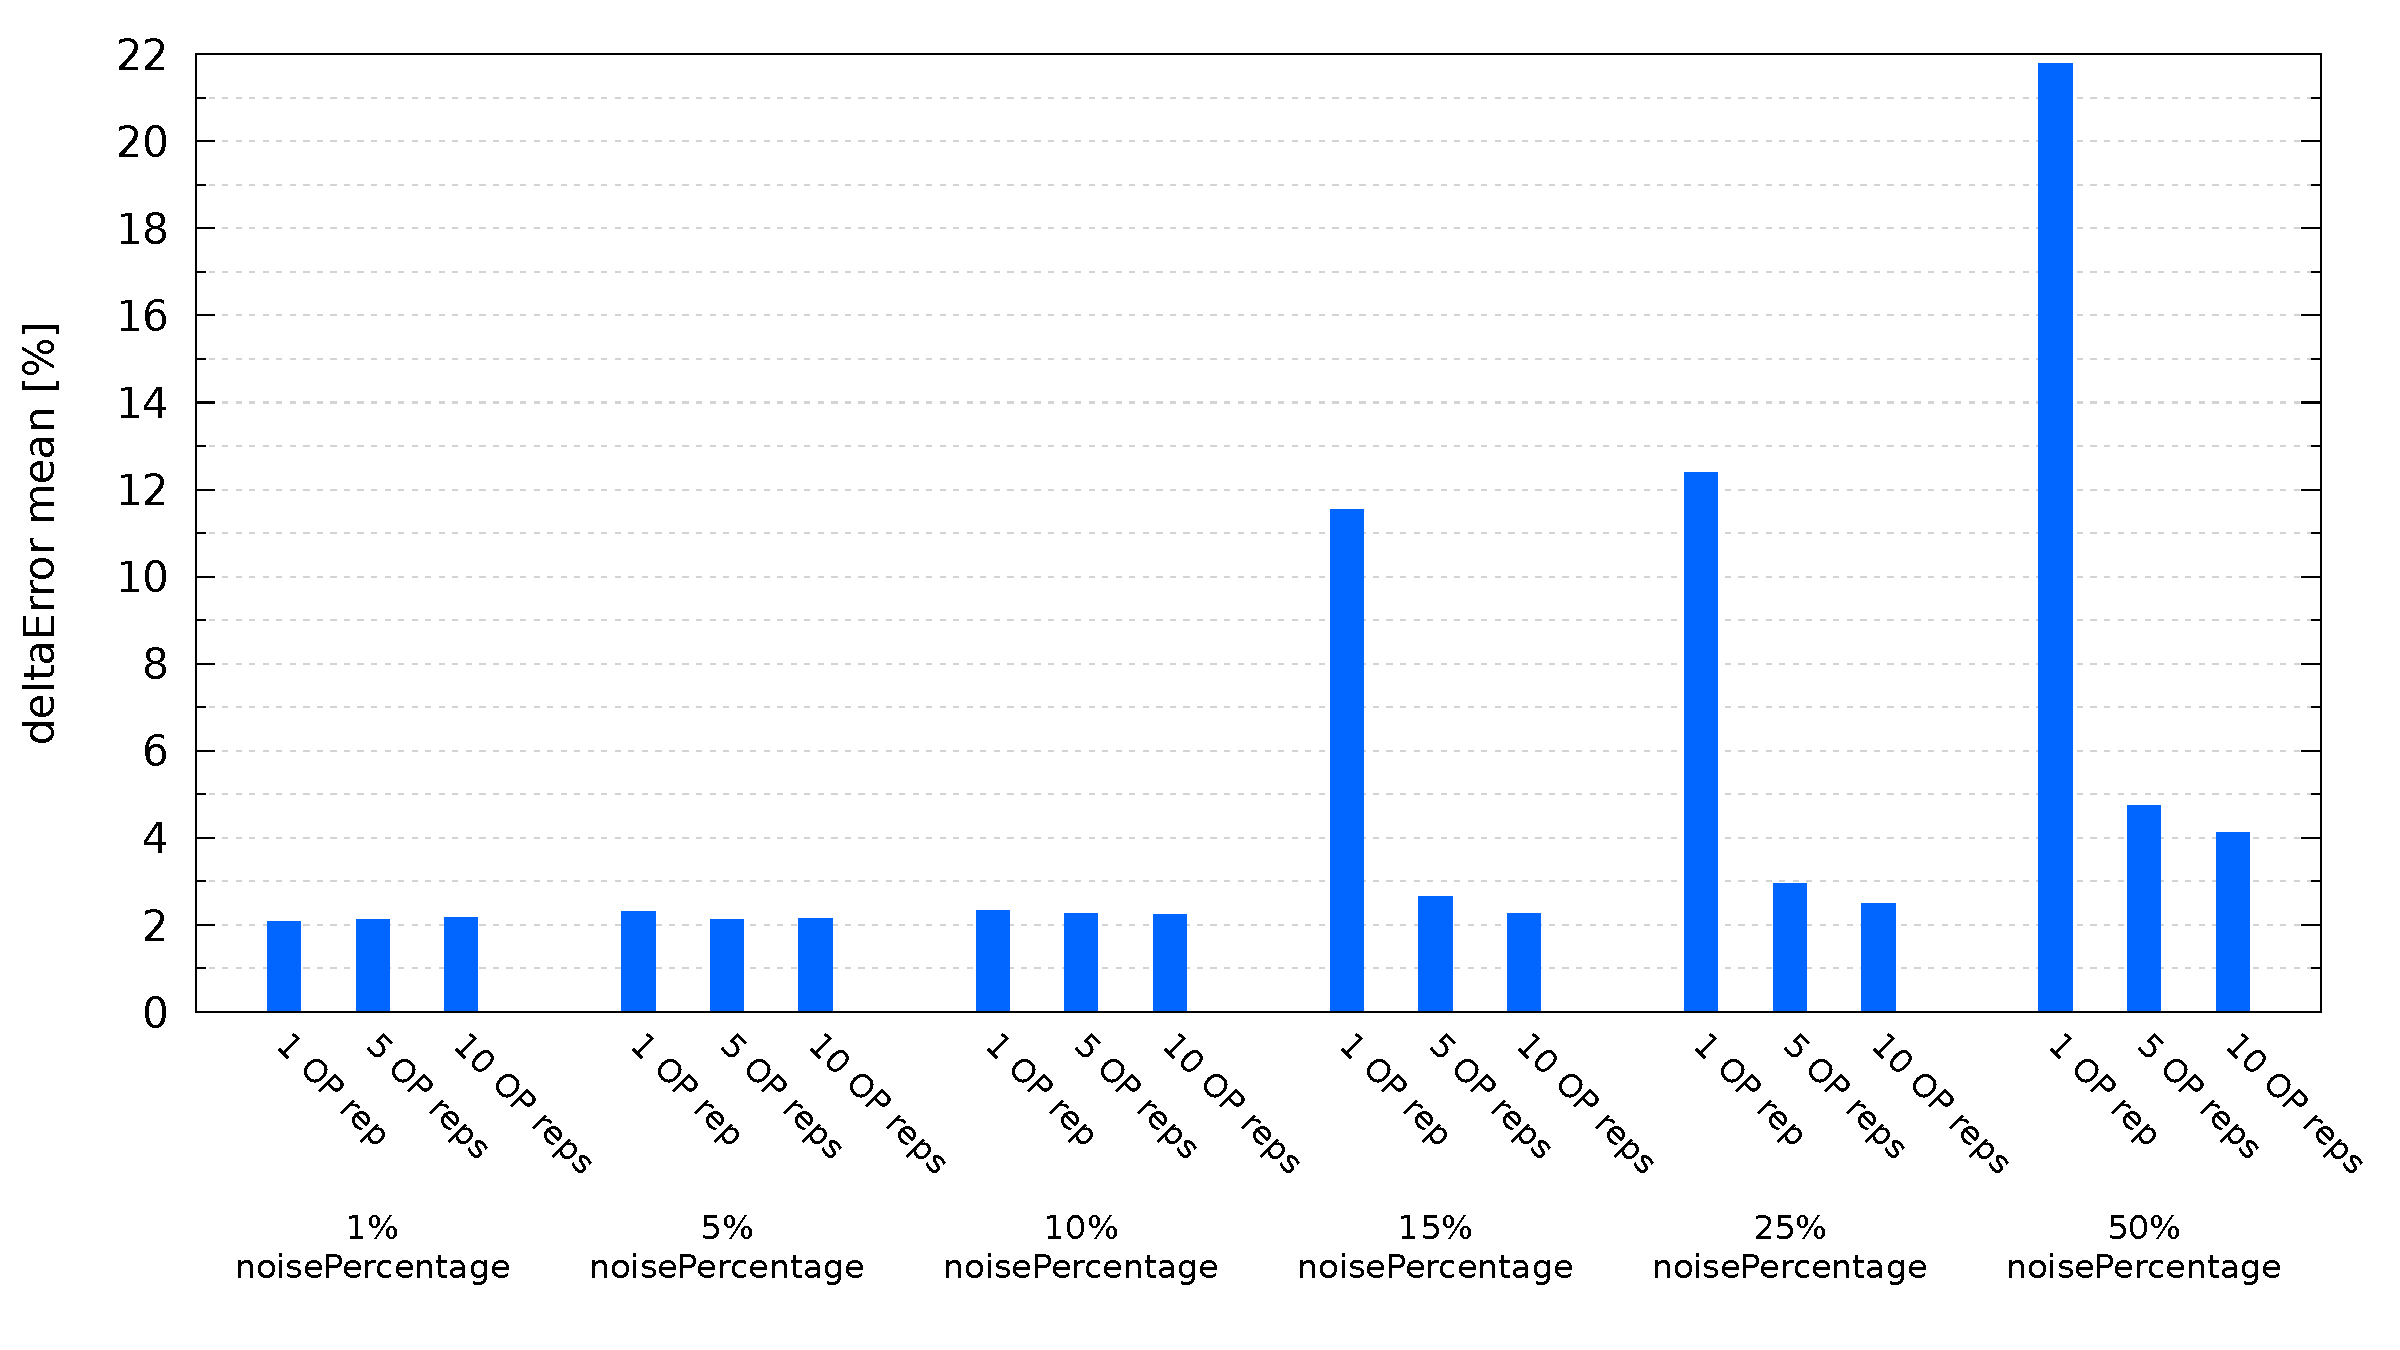
\includegraphics[width = \textwidth]{deltaErrorMeansSynth1spark2}
    
    \caption{$deltaError$ mean for throughput metric of synthetic application version 1 by varying the noisePercentage and the number of OP repetitions. Used RSM: 2nd version of implemented GLR ("polynomial combinations of degree 2")}
    
    \label{fig::synth1spark2::means}
    
\end{figure}





\begin{figure}[h]

    \centering
    
    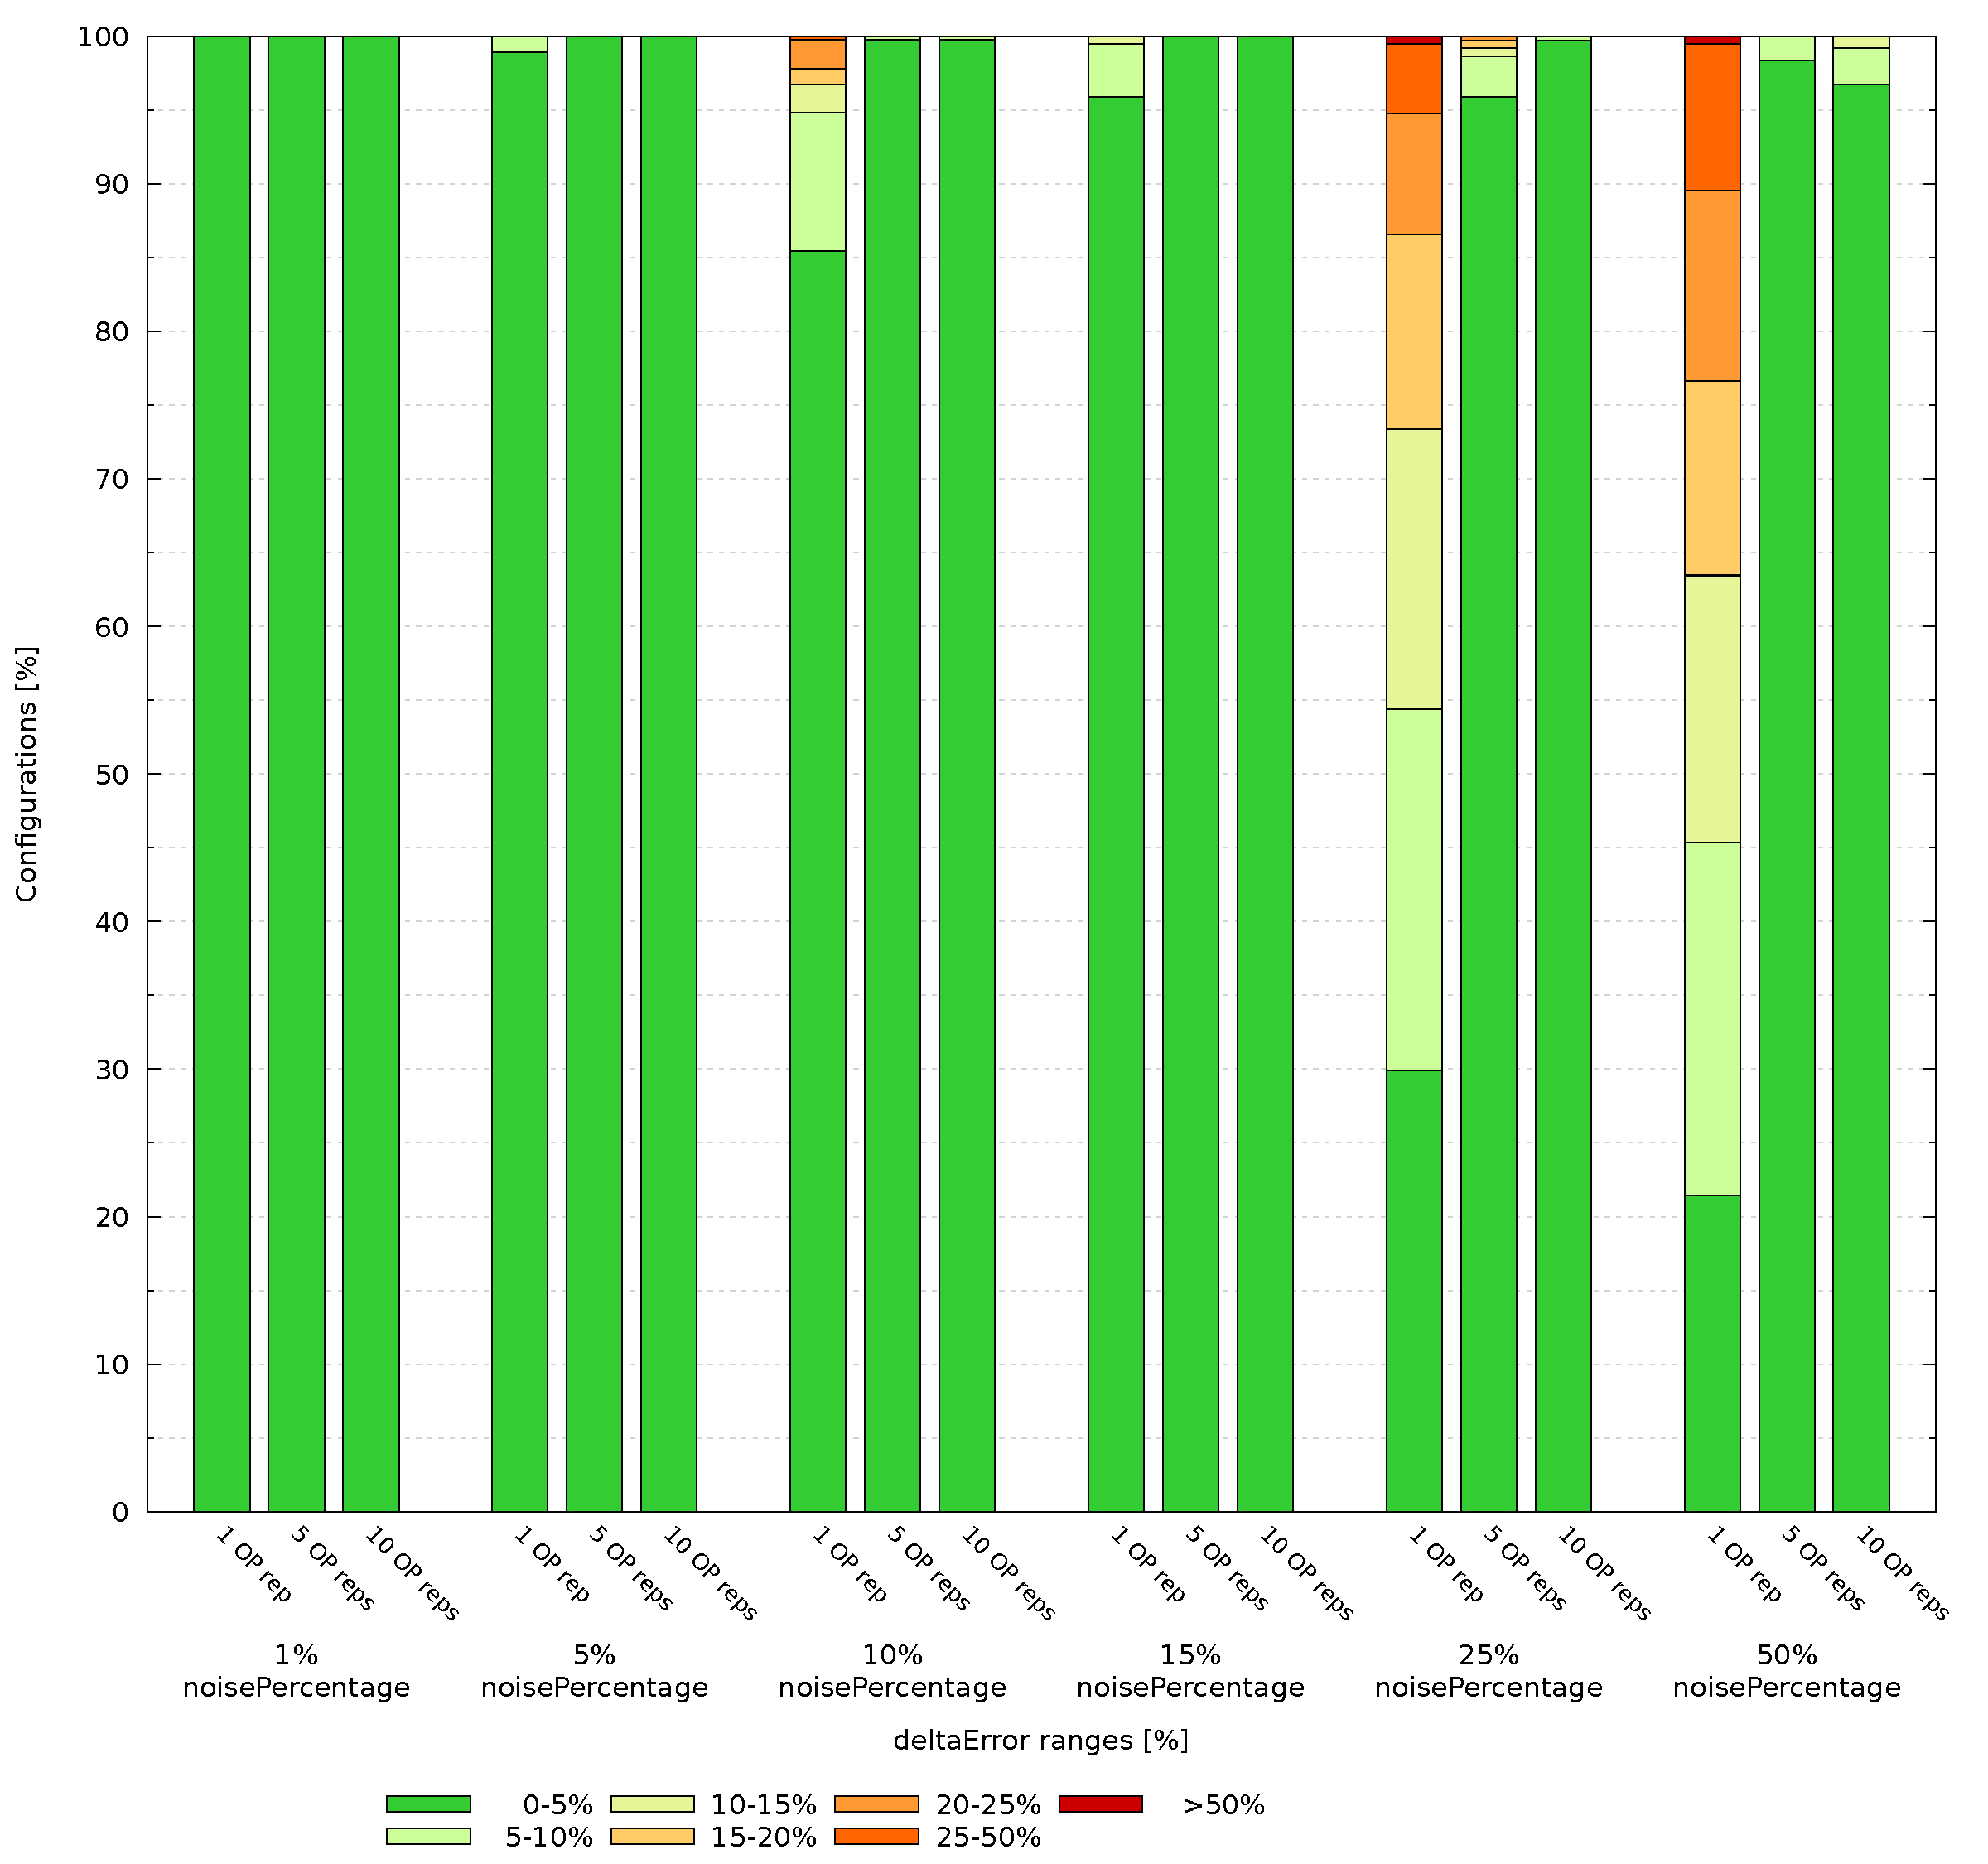
\includegraphics[width = \textwidth]{deltaErrorRangesSynth2spark2}
    
     \caption{$deltaError$ results for throughput metric of synthetic application version 2 by varying the noisePercentage and the number of OP repetitions. Used RSM: 2nd version of implemented GLR ("polynomial combinations of degree 2")}
    
    \label{fig::synth2spark2::intervals}
    
\end{figure}

\begin{figure}[h]

    \centering
    
    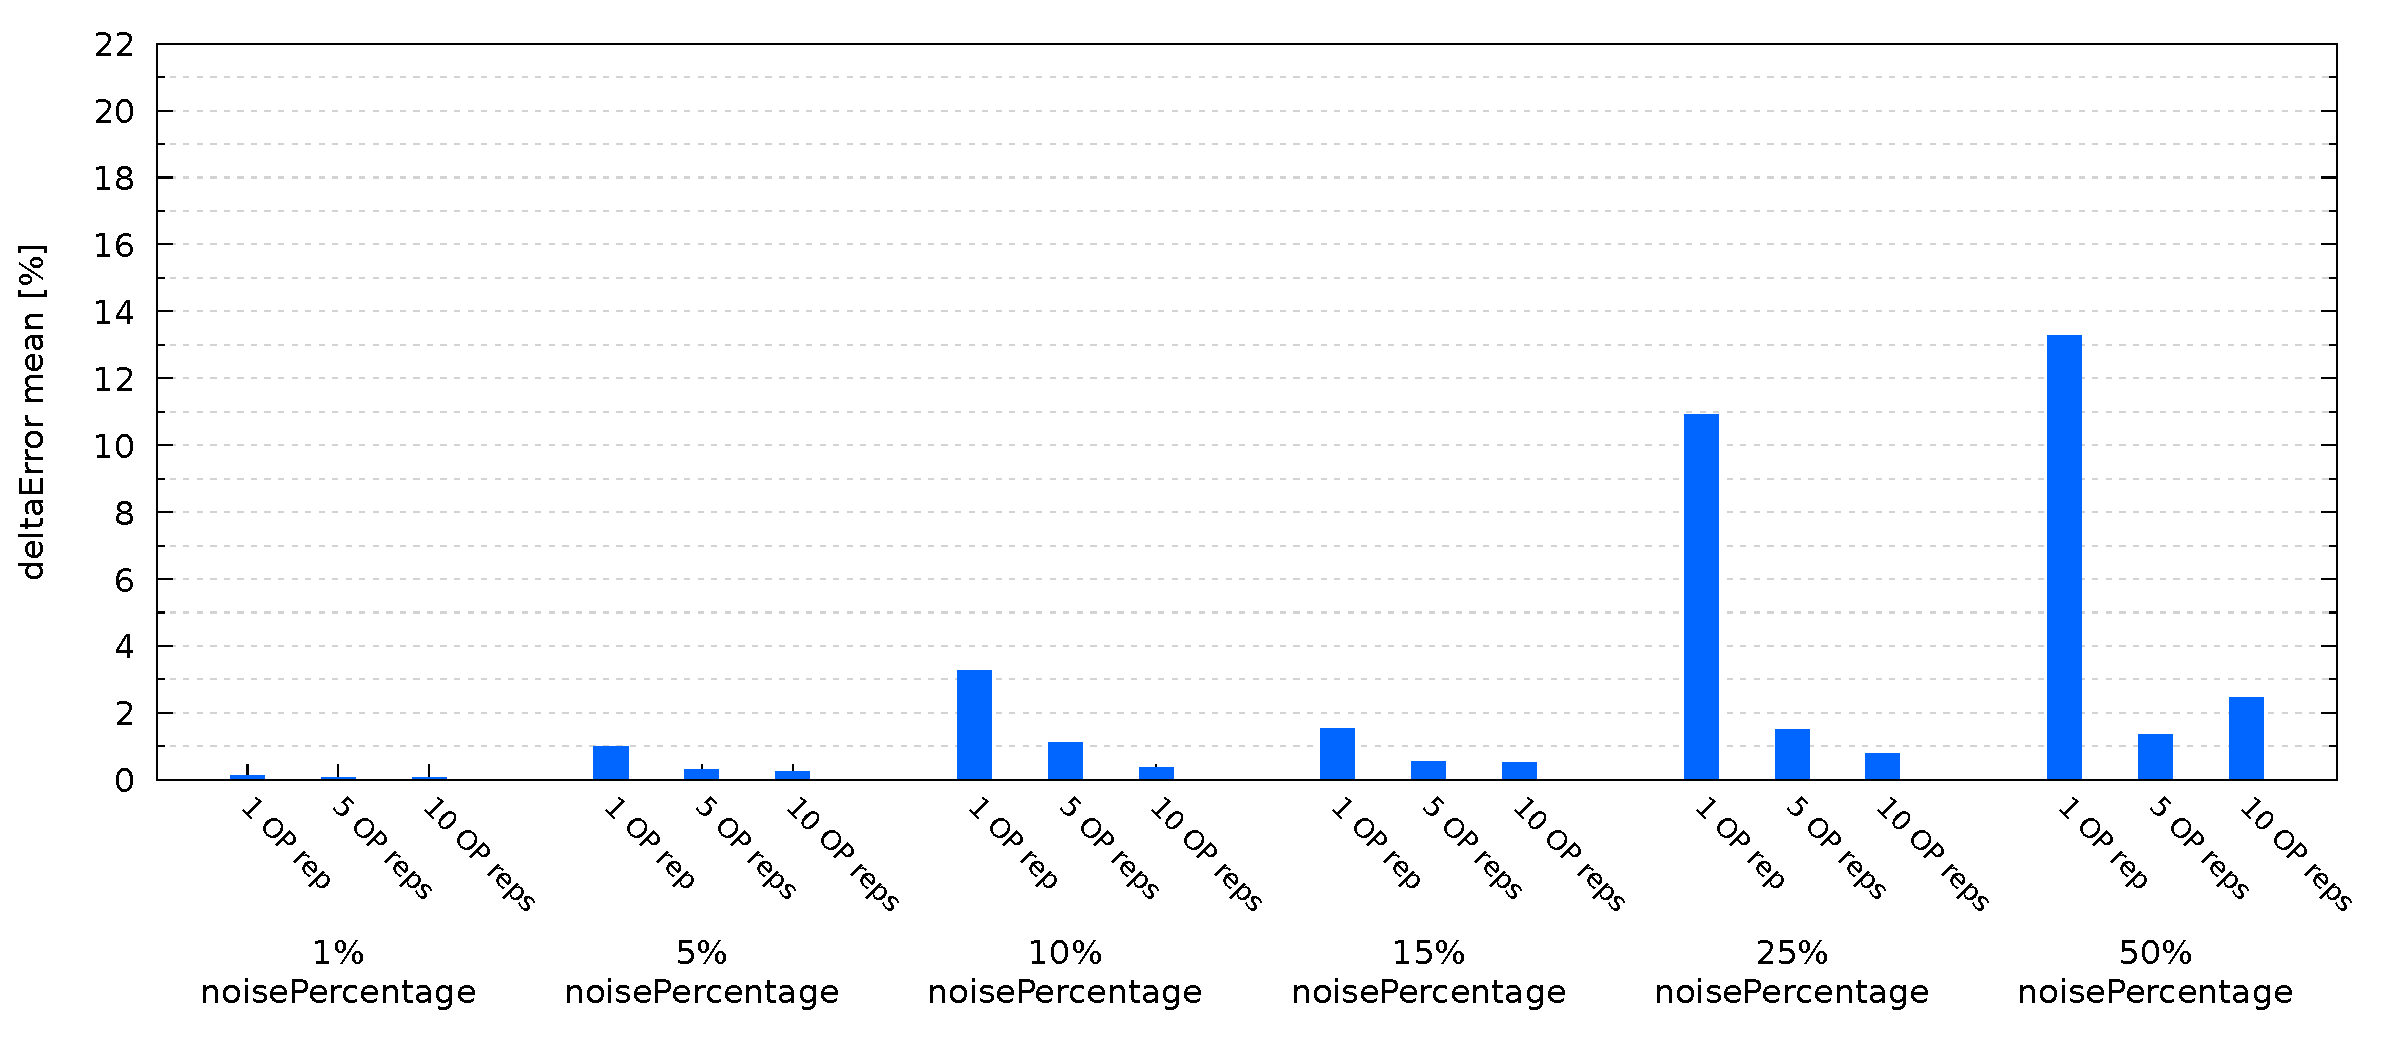
\includegraphics[width = \textwidth]{deltaErrorMeansSynth2spark2}
    
    \caption{$deltaError$ mean for throughput metric of synthetic application version 2 by varying the noisePercentage and the number of OP repetitions. Used RSM: 2nd version of implemented GLR ("polynomial combinations of degree 2")}
    
    \label{fig::synth2spark2::means}
    
\end{figure}





In Figures \ref{fig::synth1spark1::intervals}, \ref{fig::synth1spark2::intervals} and \ref{fig::synth2spark2::intervals}, each stacked bar chart represent an application setting with respect to $noisePercentage$ value and the number of repetitions, for each DoE configuration, collected during DSE phase; on y-axis there are the number of predicted OPs, in percentage, grouped with respect to measured $deltaError$ of related throughput metric; related Figures \ref{fig::synth1spark1::means}, \ref{fig::synth1spark2::means} and \ref{fig::synth2spark2::means} show $deltaError$ mean for each program setting.

From figure \ref{fig::synth1spark1::intervals} we can see that, until $noisePercentage = 15\%$, model prediction is really precise even with only 1 repetition for each DoE configuration: almost the totality of OPs have a $del\-ta\-Er\-ror$ below $5\%$; with 5 repetitions and 10 repetitions, all configurations have a $del\-ta\-Er\-ror$ below $5\%$. With the introduction of a strong noise weight, $25\%$ and $50\%$, prediction get worse with 1 OP repetition, even if, respectively, around $70\%$ and $60\%$ of configurations remains with a \textit{deltaError} below $10\%$; prediction gets back really accurate with 5 and 10 OP repetitions also with these high noise values.

Figure \ref{fig::synth1spark2::intervals} shows that, for synthetic application 1, 2nd version of the implemented GLR produces, in general, results less precise that the ones generated with the 1st GLR version: up to $noisePercentage = 10\%$, quality of predicted models is very satisfying, where more than $90\%$ of OPs have a $deltaError$ below $5\%$; from noise weight equal to $15\%$, $25\%$, $50\%$ and with 1 OP repetition, this $deltaError$ percentage decreases to $35\%$, $30\%$ and $15\%$ respectively and a visible number of Operating Points has a $deltaError$ greater that $25\%$; for these settings, model prediction quality remarkably increases collecting more training data for each Design of Experiments configuration: with 5 and 10 OP repetitions we notice very few predicted OPs with a $deltaError$ greater that $10\%$, so prediction quality becomes very accurate even in these awful cases.

Concerning synthetic application version 2 with the 2nd version of implemented Generalized Linear Regression as RSM (figure \ref{fig::synth2spark2::intervals}), results are very similar to the ones related to synthetic application version 1 with 1st version of implemented Generalized Linear Regression (figure \ref{fig::synth1spark1::intervals}): quality of model prediction is generally very high, even with heavy noises but, in these cases, there is the need of more OP repetitions in order to mitigate this strong disturbance.

For synthetic application version 1, as it can be understood, 1st implemented version of GLR works slightly better than the 2nd one, but their prediction times are very different, as shown in table \ref{tab::GLRtimes}:

\begin{table}[h]

    \centering
    
    \begin{tabular}{cccc}
    
        \toprule
         & 1 OP rep & 5 OP reps & 10 OP reps \\
        \midrule
        GLR 1st version & 155.52 sec & 155.7 sec & 157.72 sec \\
        GLR 2nd version & 23.21 sec & 23.64 sec & 23.8 sec \\
        \bottomrule 
    
    \end{tabular}

    \caption{Model prediction times for each implemented Generalized Linear Regression for each number of OP repetitions scenario}
    \label{tab::GLRtimes}
    
\end{table}

2nd GLR version takes less than 24 seconds to predict complete model, while 1st GLR version approximately 156 seconds: the former, almost to the same level of quality, is more than 6 times faster than the latter. Moreover, we have noticed that the number of OP repetitions affects very poorly model prediction time: from table \ref{tab::GLRtimes} we can understand that, among 1, 5 and 10 OP repetitions for each DoE configuration case, times vary very few.

We have not disclosed model prediction quality for synthetic application version 2 with the 1st implemented version of GLR: \textit{"transformations by functions"} strategy is not able to capture functions of second order behavior, as variable $executionTime$ is built in this case. On the contrary, \textit{"polynomial expansion of second order"} technique has the capability to highly predict functions with, for instance, logarithmic or square root values, as demonstrated in the second model prediction analysis (figure \ref{fig::synth1spark2::intervals}).

From last analyses, we can assert that Generalized Linear Regression with \textit{"polynomial expansion of second order"} is a Response Surface Methodology much more powerful than GLR that uses \textit{"transformations by functions"}: the latter version can predict a restricted set of scenarios, while the former is able to include those cases and the wide variety of quadratic functions. Agorà has been able to predict very well these metric behaviors and to properly manage strong noise disturbances, with the necessity to do, in some cases, a longer Design Space Exploration phase, collecting more OPs for each Design of Experiments configuration; lastly, figures \ref{fig::synth1spark1::means}, \ref{fig::synth1spark2::means} and \ref{fig::synth2spark2::means} recap all various scenarios, showing $deltaError$ mean values that increase with high noises, going back still very low with 5 and 10 OP repetitions, even in the worst cases.


\subsubsection{Execution times}

Concerning execution times, we want to show the significant benefit of sharing Design Space Exploration phase among several nodes, running the same application: the 2nd version of synthetic application with $noise\-Percentage = 10\%$ is executed, using Face Centered Central Composite Desing of Experiments with one Center Point and collecting, for each configuration, 20 repetitions; for this application setting, the total number of configurations to be explored is 300. We accomplish this DSE phase with 1 up to 10 executing applications, collecting the overall executing time, represented by each bar chart in Figure \ref{fig::DSEtimes}.

\begin{figure}[h]

    \centering
    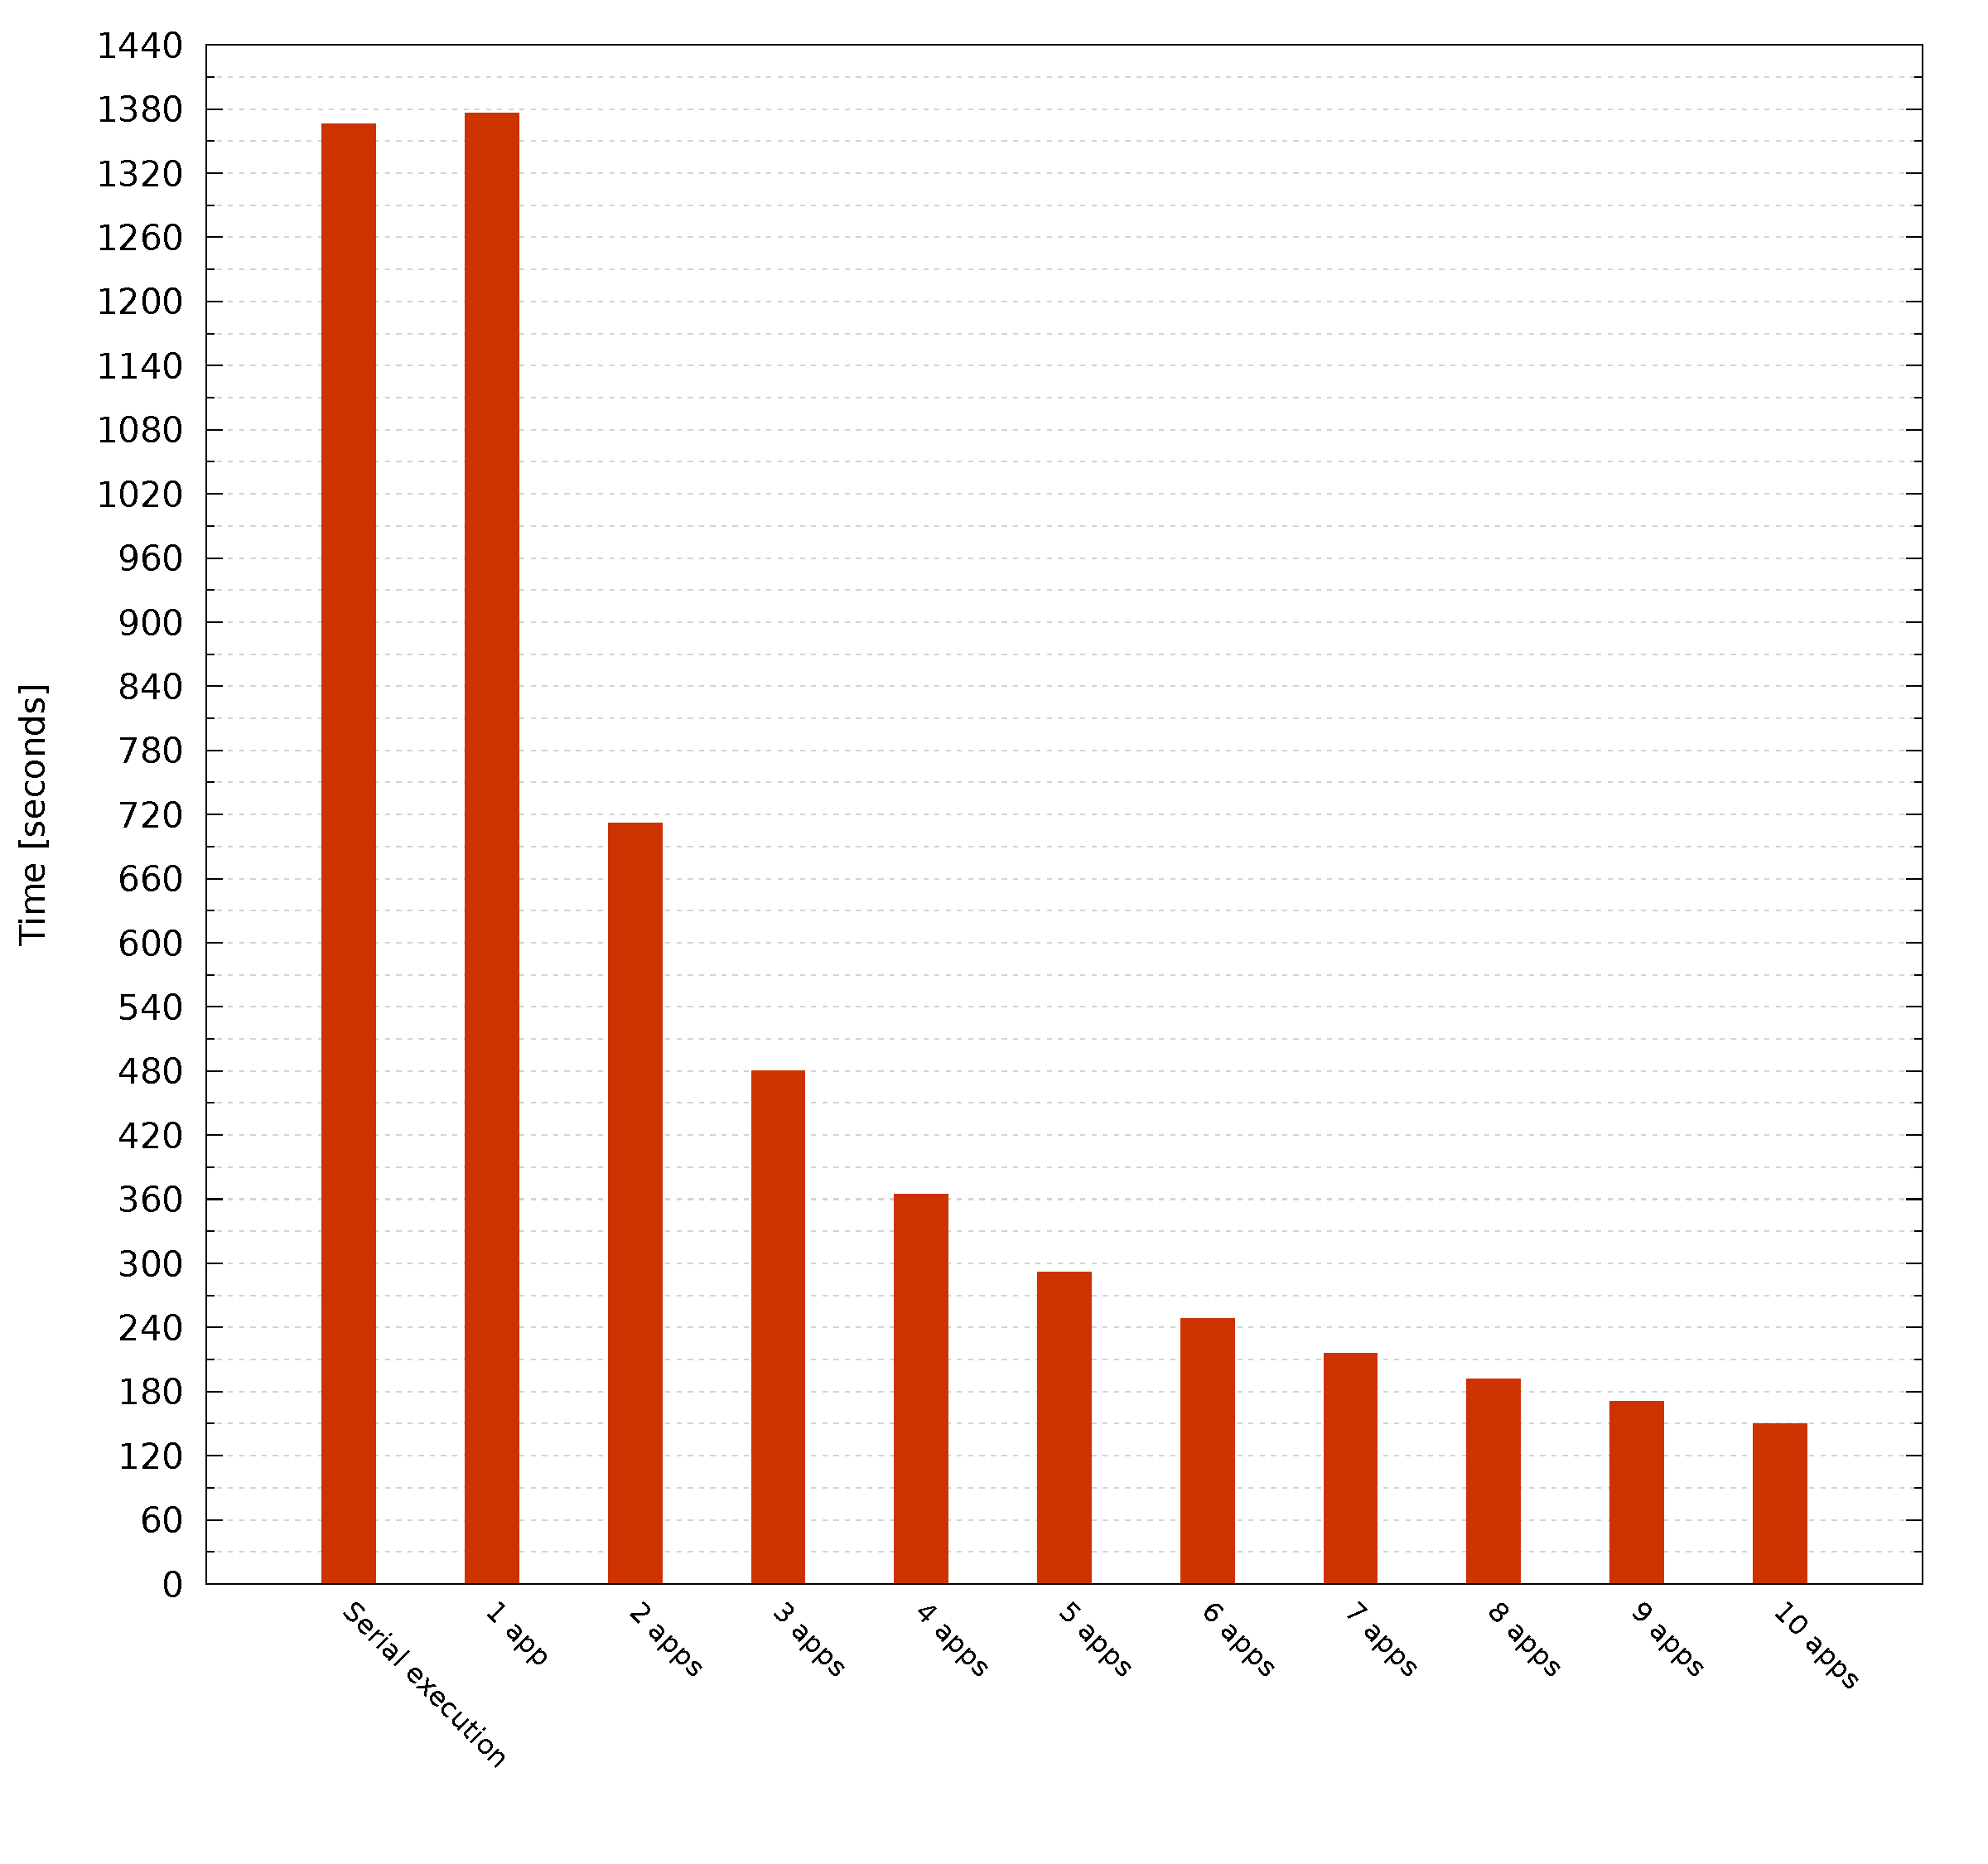
\includegraphics[width = \textwidth]{DSEtimes}
    \caption{Design Space Exploration time by varying the number of executing applications}
    \label{fig::DSEtimes}
    
\end{figure}

From figure \ref{fig::DSEtimes} we can see that Agorà takes about 23 minutes to terminate Design Space Exploration with 1 executing application (second bar chart). The first bar chart shows the amount of time needed to execute application with all the 300 configurations in a serial way, without Agorà; this execution lasts around 10 seconds less than the first analyzed scenario, due to the lack of Agorà overheads; as we can understand, they are in any case very little: they add only approximately $0.73\%$ of time with respect of the serial execution. From 2 executing applications on, DSE time strongly decreases: Agorà takes around 12 minutes to finish this phase with just 2 executing applications, 8 minutes with 3 ones, up to only 2 and a half minutes with 10 ones, more than 9 times lower than DSE phase with 1 application. Sharing Design Space Exploration phase among more than one executing application clearly speeds up overall time, since collection of training data duration, that is much longer than model prediction one (reported in table \ref{tab::GLRtimes}), considerably goes down.

Now we want to show general Agorà advantages, comparing a Full-Factorial, so exhaustive, application execution with the one supervised by this work; in figure \ref{fig::full_cris}, first bar chart shows overall time needed to compute Full-Factorial run for synthetic application version 2 with $noisePercentage = 15\%$, analyzing every possible configuration one time; next stacked bar charts show overall time, divided by DSE phase and model prediction, for the same application setting using Agorà and collecting 1, 5 and 10 OP repetitions for each DoE configuration:

\begin{figure}[h]

    \centering
    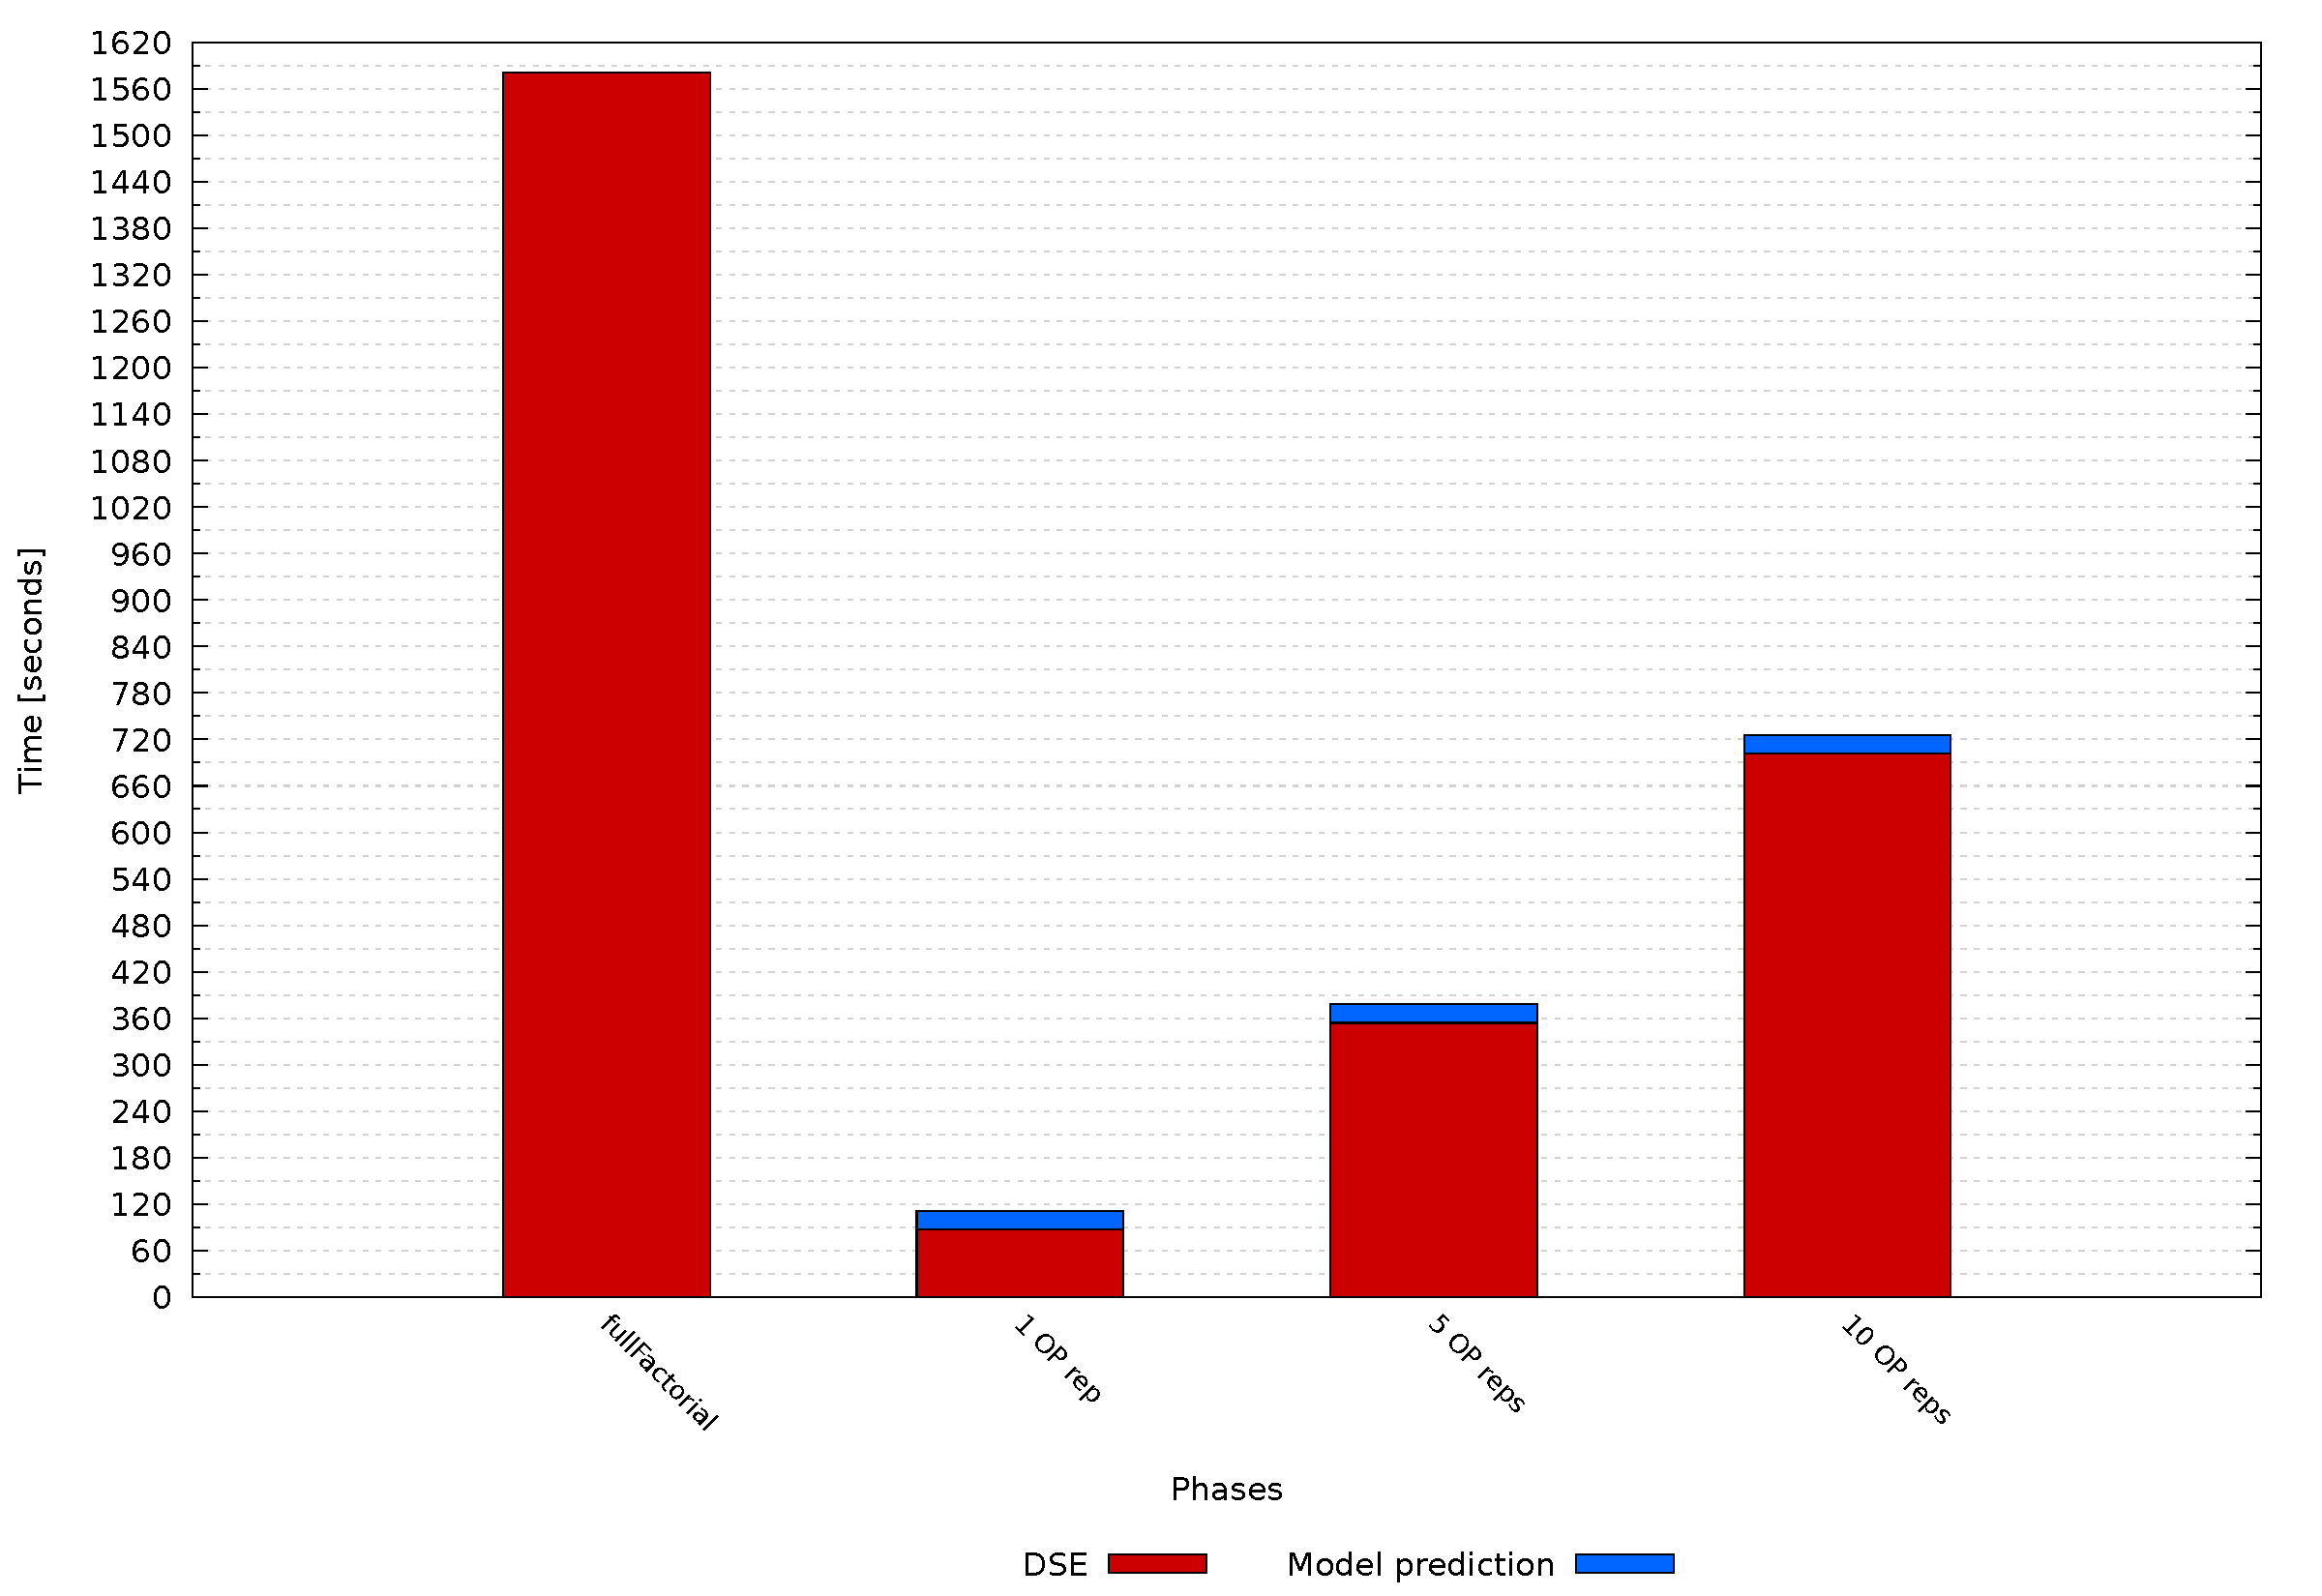
\includegraphics[width = \textwidth]{fullFactorial_tesiCris}
    \caption{Execution time for different synthetic application version 2 settings}
    \label{fig::full_cris}
    
\end{figure}

Figure \ref{fig::full_cris} shows that an exhaustive execution of analyzed application takes more than 26 minutes to finish; with the introduction of Agorà, using Face Centered Central Composite Desing of Experiments with one Center Point and the 2nd version of implemented GLR as RSM, overall time becomes 12 minutes if 10 repetitions for each DoE configuration are collected, about 6 minutes with 5 repetitions and even around 2 minutes with 1 repetition; we specify that, if we want to explore every possible configuration in the exhaustive analysis as much as we do for 5 and 10 OP repetitions of DoE configurations with Agorà, of course overall time is 130 minutes and 260 minutes respectively (5 times and 10 times the shown serial execution time), increasing much more the gap between Full-Factorial execution and the ones with the supervise of this work. Finally, we also want to remind, from figures \ref{fig::synth2spark2::intervals} and \ref{fig::synth2spark2::means}, that Agorà, for this application setting, can predict a complete model with a very high quality even collecting just 1 repetition for each DoE configuration, so the final result is very similar to an exhaustive analysis. Therefore, this work can produce high benefits in the prediction of application complete model, starting from a small subset of configurations.


\subsubsection{Application behavior over time}

Last figure wants to show application behavior during execution with the supervise of Agorà and mARGOt autotuner; on x-axis there is time, while on y-axis there are observed metric of interest values during execution. We have run synthetic application version 2 with $noisePercentage = 15\%$, using Face Centered Central Composite Design of Experiments with one Center Point and the 2nd version of implemented GLR as RSM, collecting 5 repetitions for each Design of Experiments configuration during DSE phase; objective functions have been set up to $Throughput > 3$ and $Error < 1$; figure \ref{fig::appBeh} shows results:

\begin{figure}[h]

    \centering
    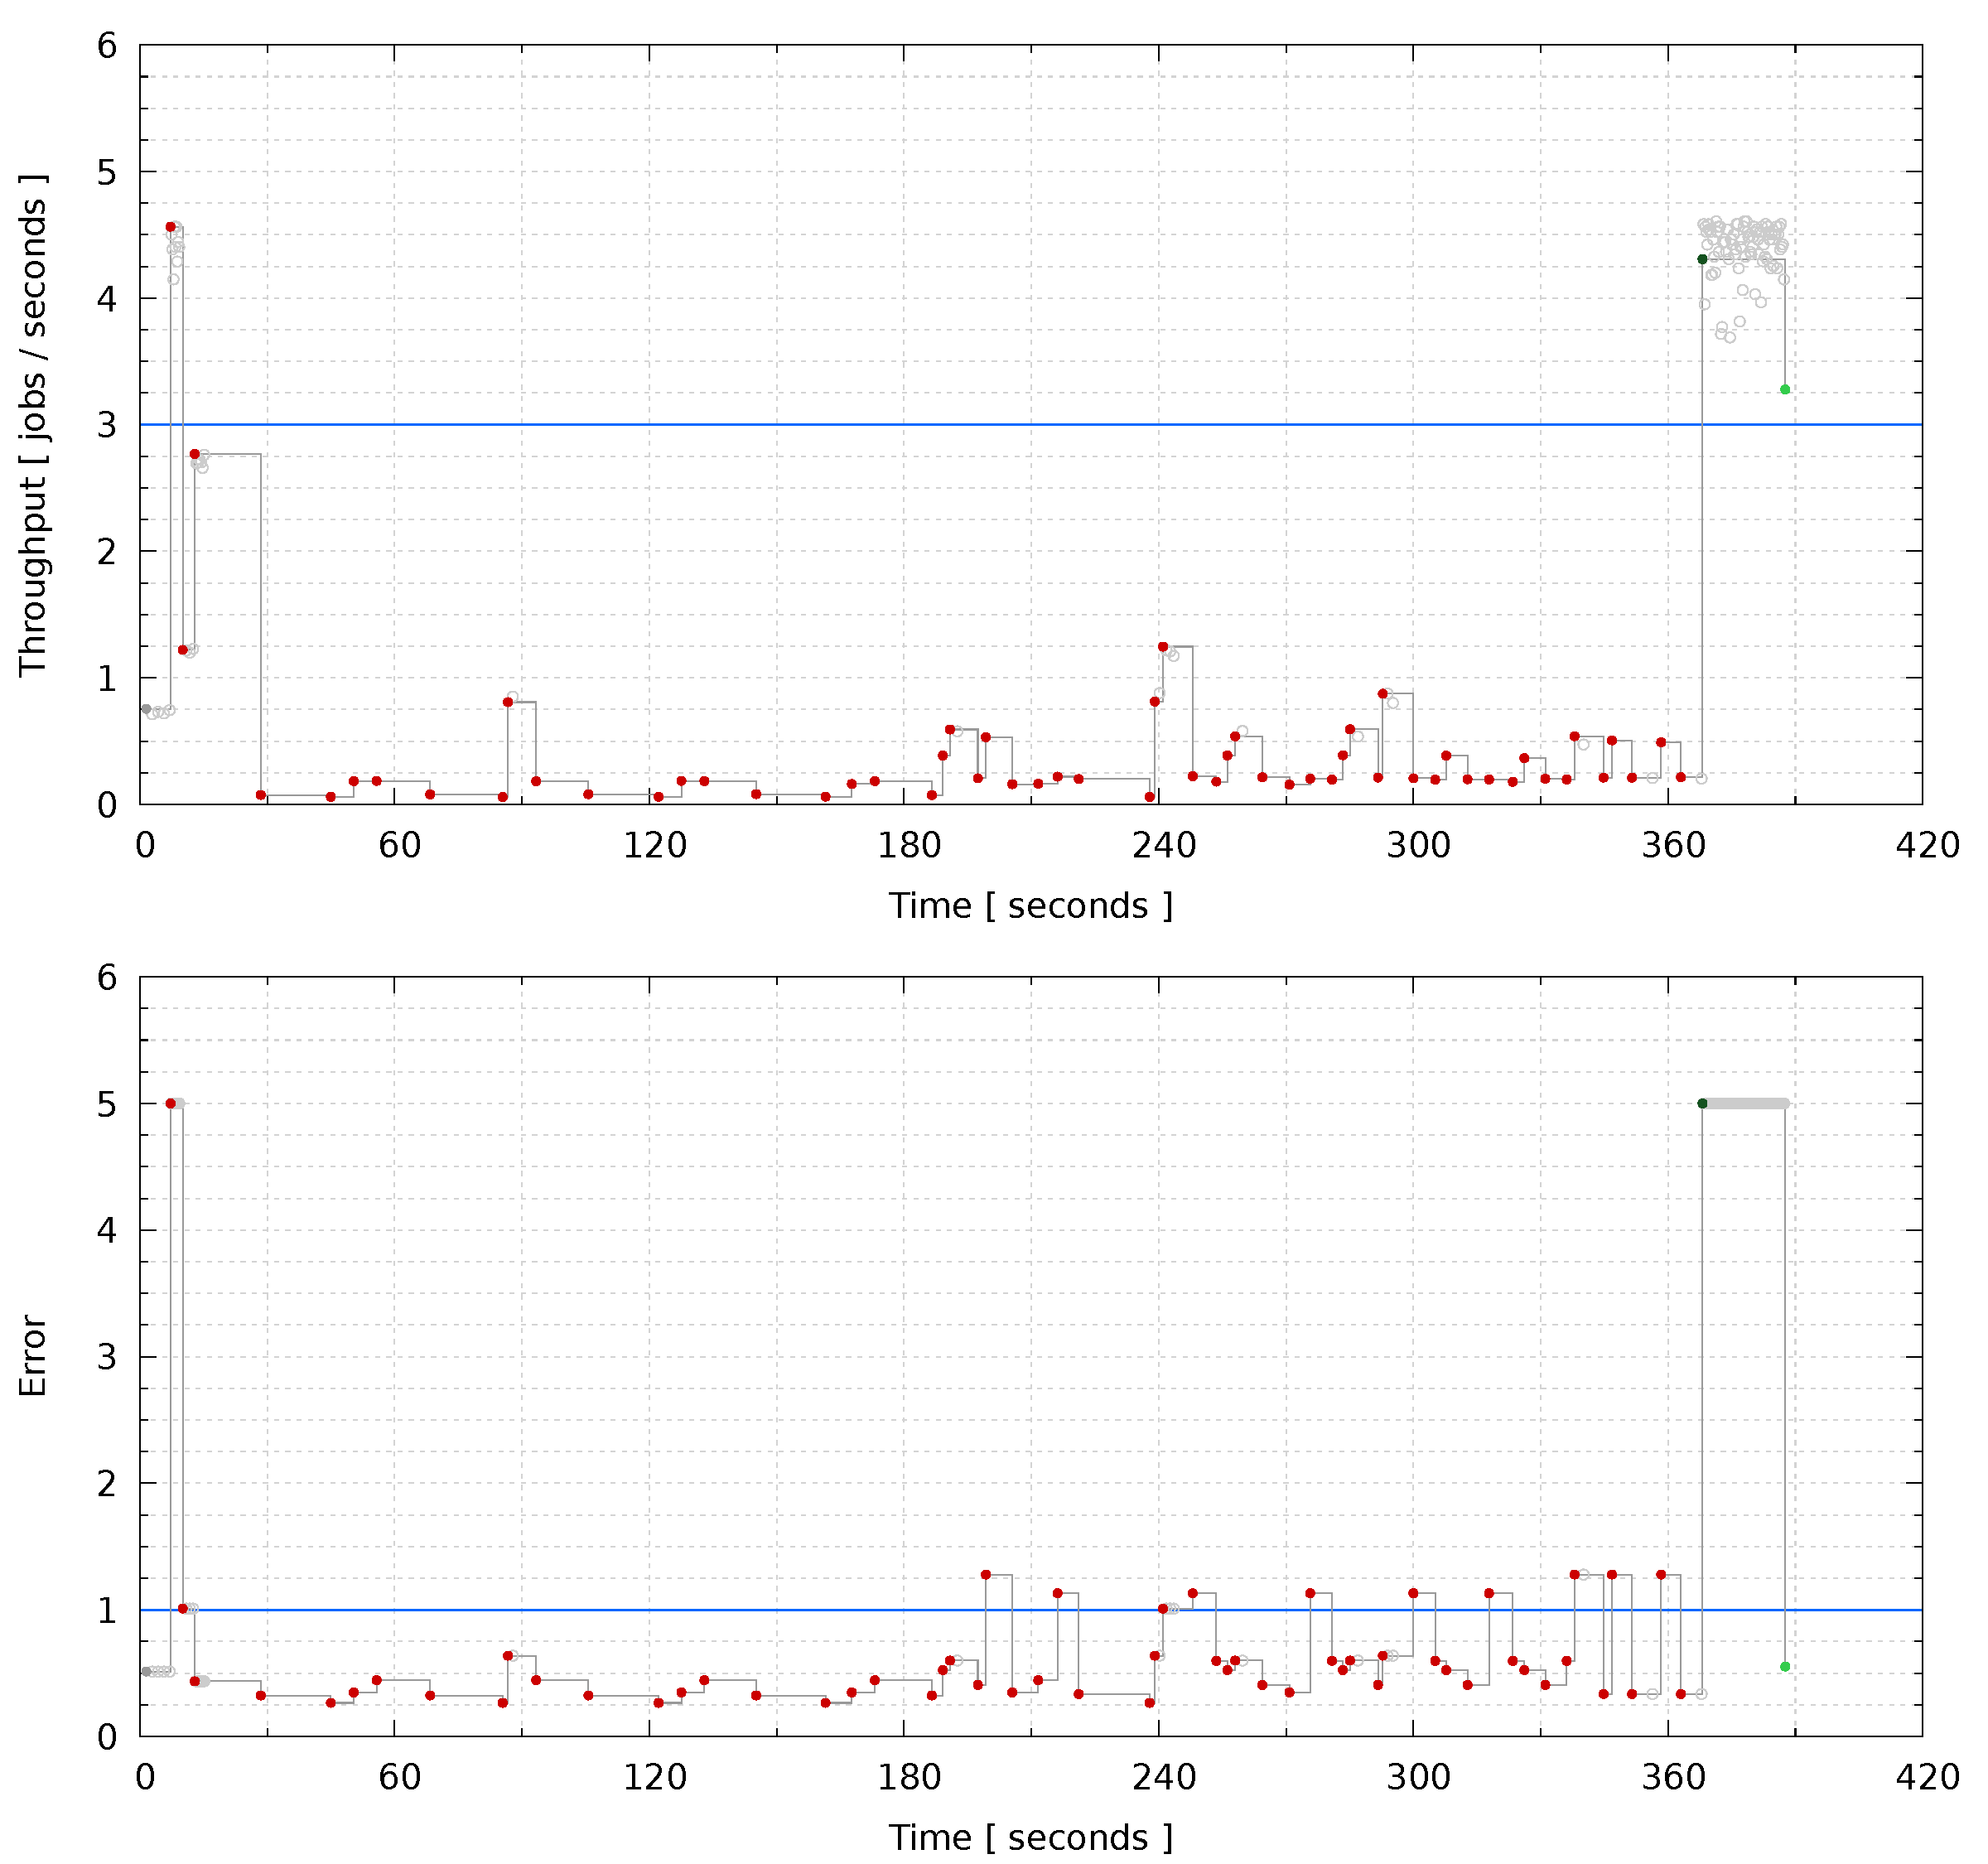
\includegraphics[width = \textwidth]{appBehavior}
    \caption{Metric values by varying time}
    \label{fig::appBeh}
    
\end{figure}

Every couple of corresponding points in graphs of figure \ref{fig::appBeh} represents a configuration with which the application has been executed, obtaining certain throughput and error metric values; from a colored couple of points to the following one, the application has maintained parameter values corresponding to the former couple; grey empty couples of points indicate application execution with parameter values equal to the first previous colored couple. At the beginning, application runs with default configuration, corresponding to an error of around 0.5 and a throughput equal to about 0.75 (grey couple of points); Agorà starts Design Space Exploration, sending DoE configurations: mARGOt, from time to time, sets application parameters with these values, so observed metric of interest values vary during all this phase (red couples of points); when DSE phase terminates, Agorà sends a partial model (see \ref{DoEModelSend}) and it starts predicting the complete list of Operating Points: mARGOt chooses the best application configuration that fulfills objective functions, represented by dark green couple of points; throughput is around 4.25, so the first goal is respected, while error is about 5, so the second goal is not achieved (blue lines highlight boundaries of objective functions); when application receives the complete model (around at 6 and a half minutes after starting time), it is set with another configuration (light green couple of points): obtained throughput is approximately 3.25 and error is about 0.5, so all objective functions are fulfilled; of course, if objective functions don't change, program keeps running with this Operating Point.




\subsection{Swaptions application}

We test Agorà on a real scenario; we use Face Centered Central Composite DoE with One Center Point as Design of Experiments and the 2nd version of implemented Generalized Linear Regression as Response Surface Methodology; due to application computing kernel (Monte Carlo simulations), we have decided to collect, for each DoE configuration, a meaningful number of repetitions, setting this value to 15.


\subsubsection{Model prediction quality}

Next figures show results on predicted model using $deltaError$ measure, as done for synthetic application analysis (see \ref{deltaErrorExplanation}), for both $avg\_error$ and $avg\_throughput$ metrics:





\begin{figure}[h]

    \centering
    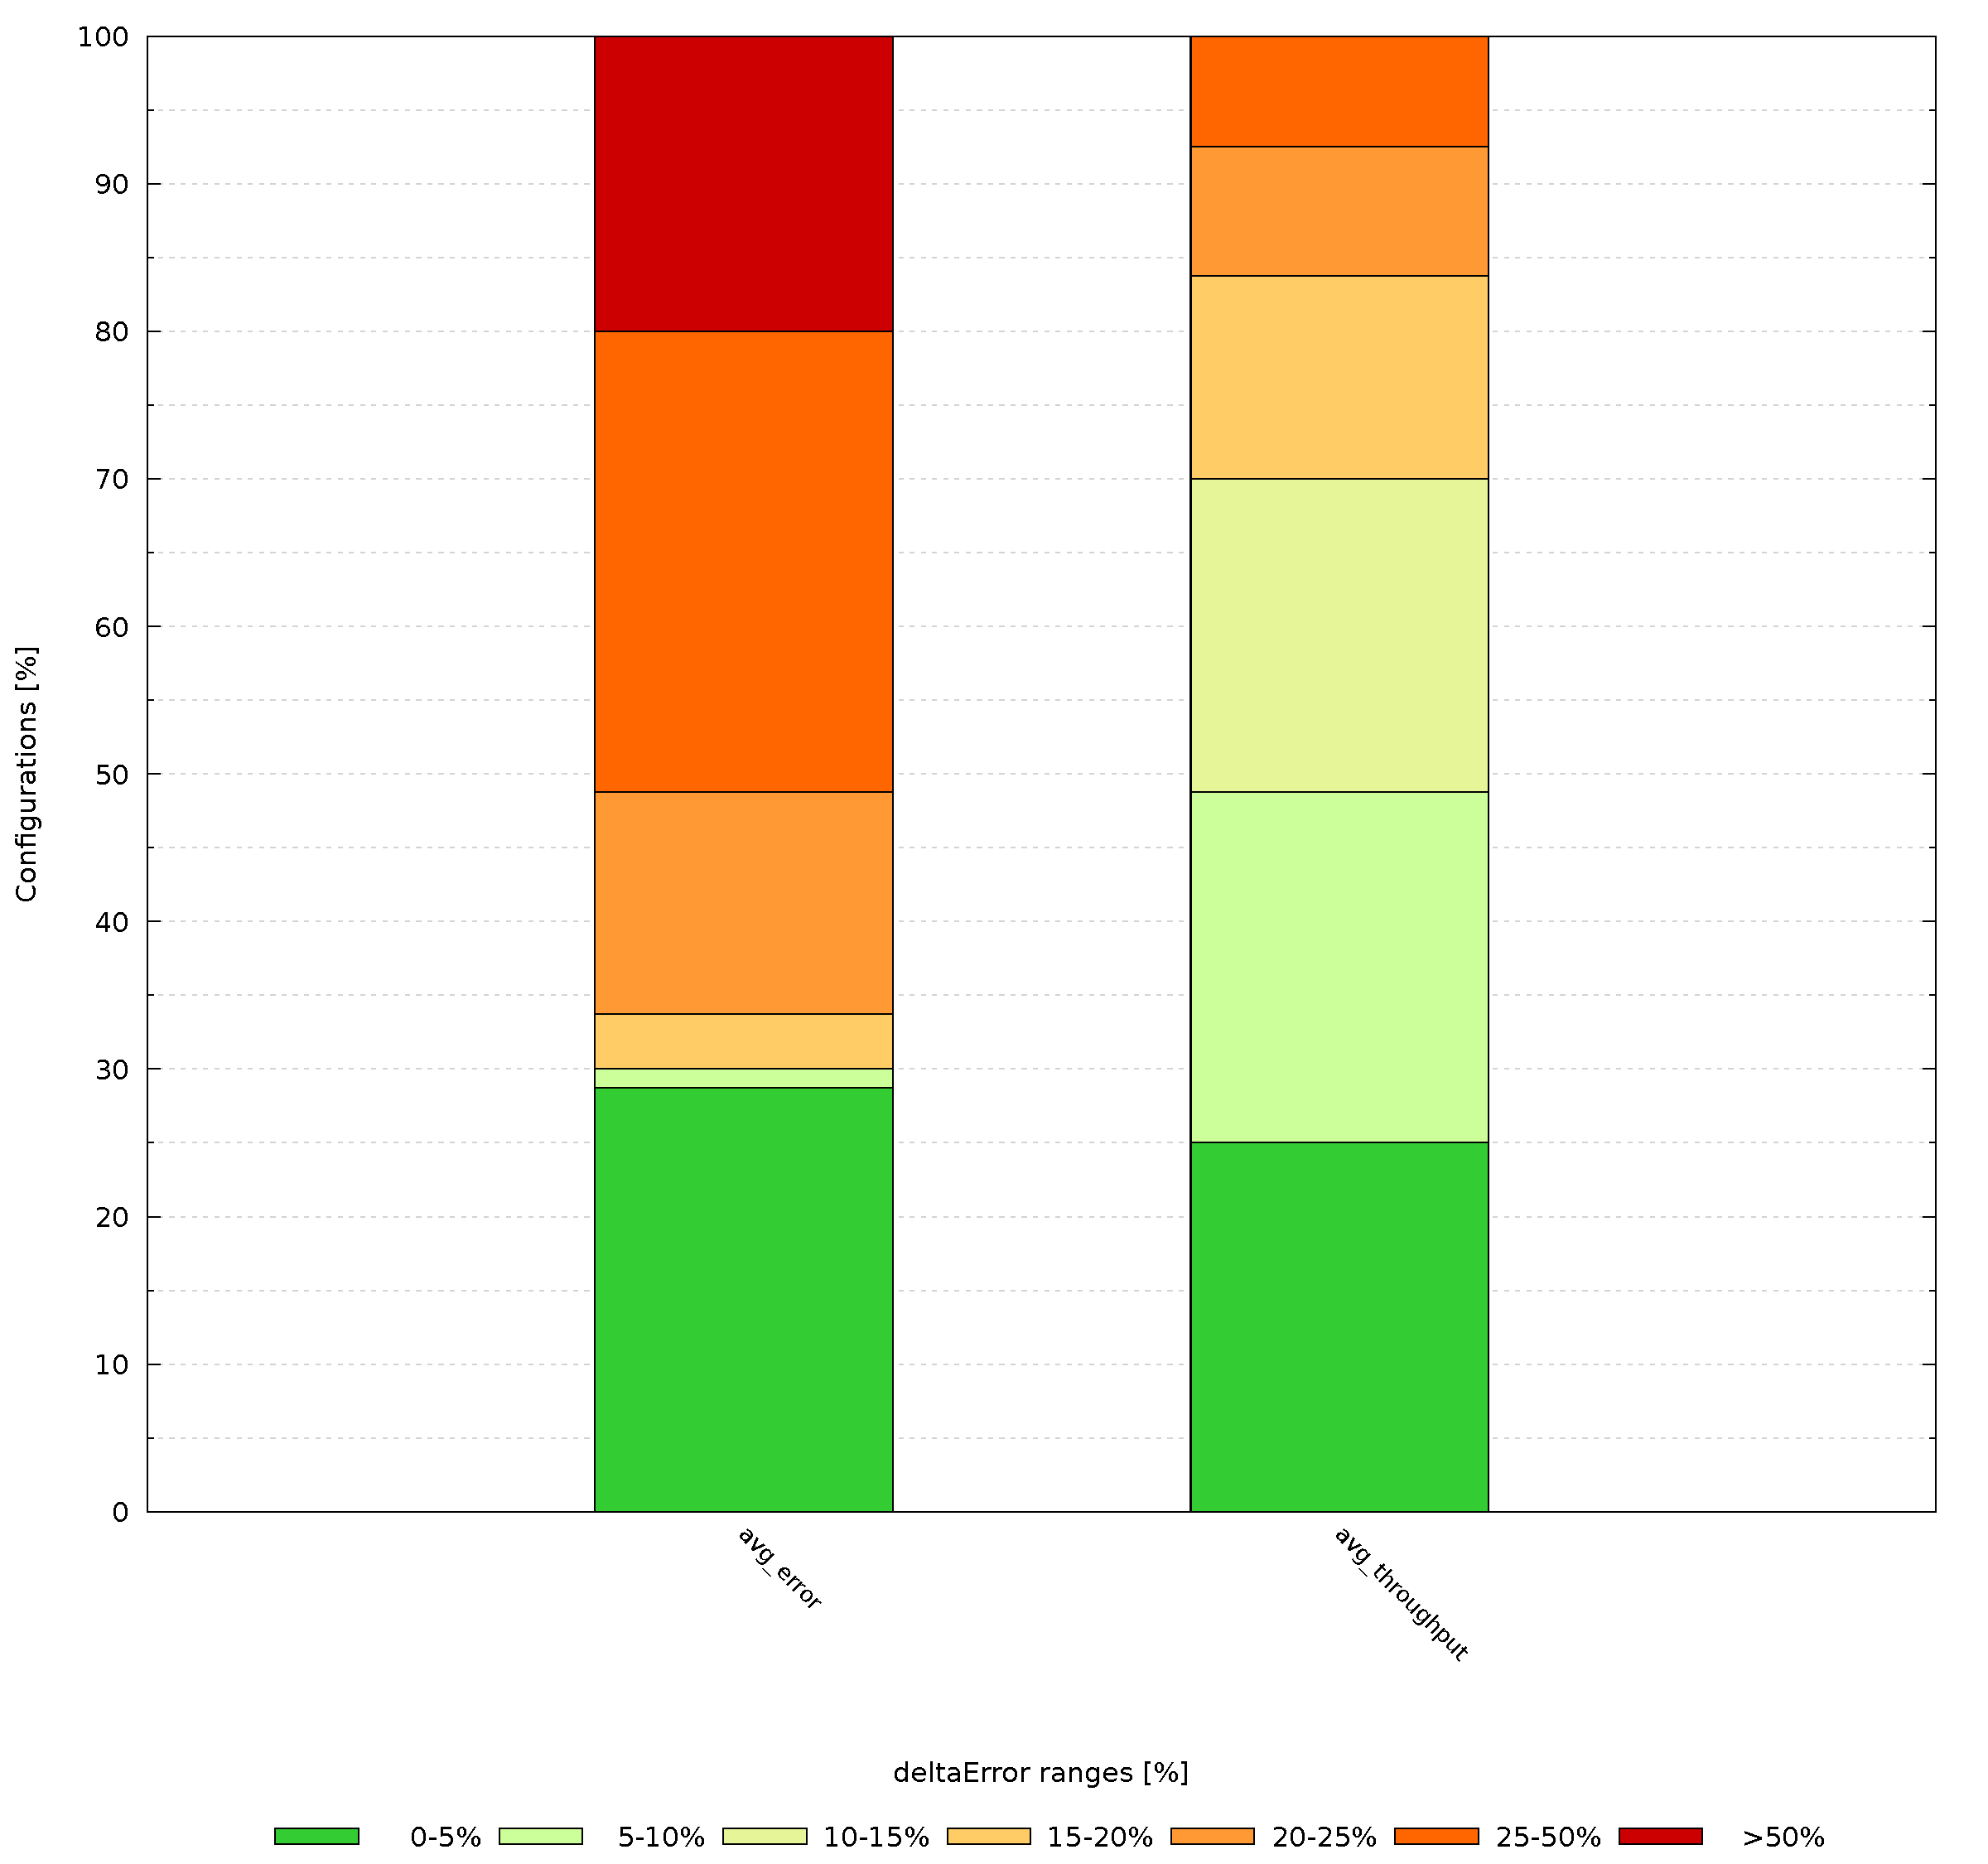
\includegraphics[width = \textwidth]{deltaErrorRangesSwaptions15Spark2}
    \caption{$deltaError$ results for both Swaptions metrics of interest}
    \label{fig::swaptions15spark2::intervals}
    
\end{figure}

\begin{figure}[h]

    \centering
    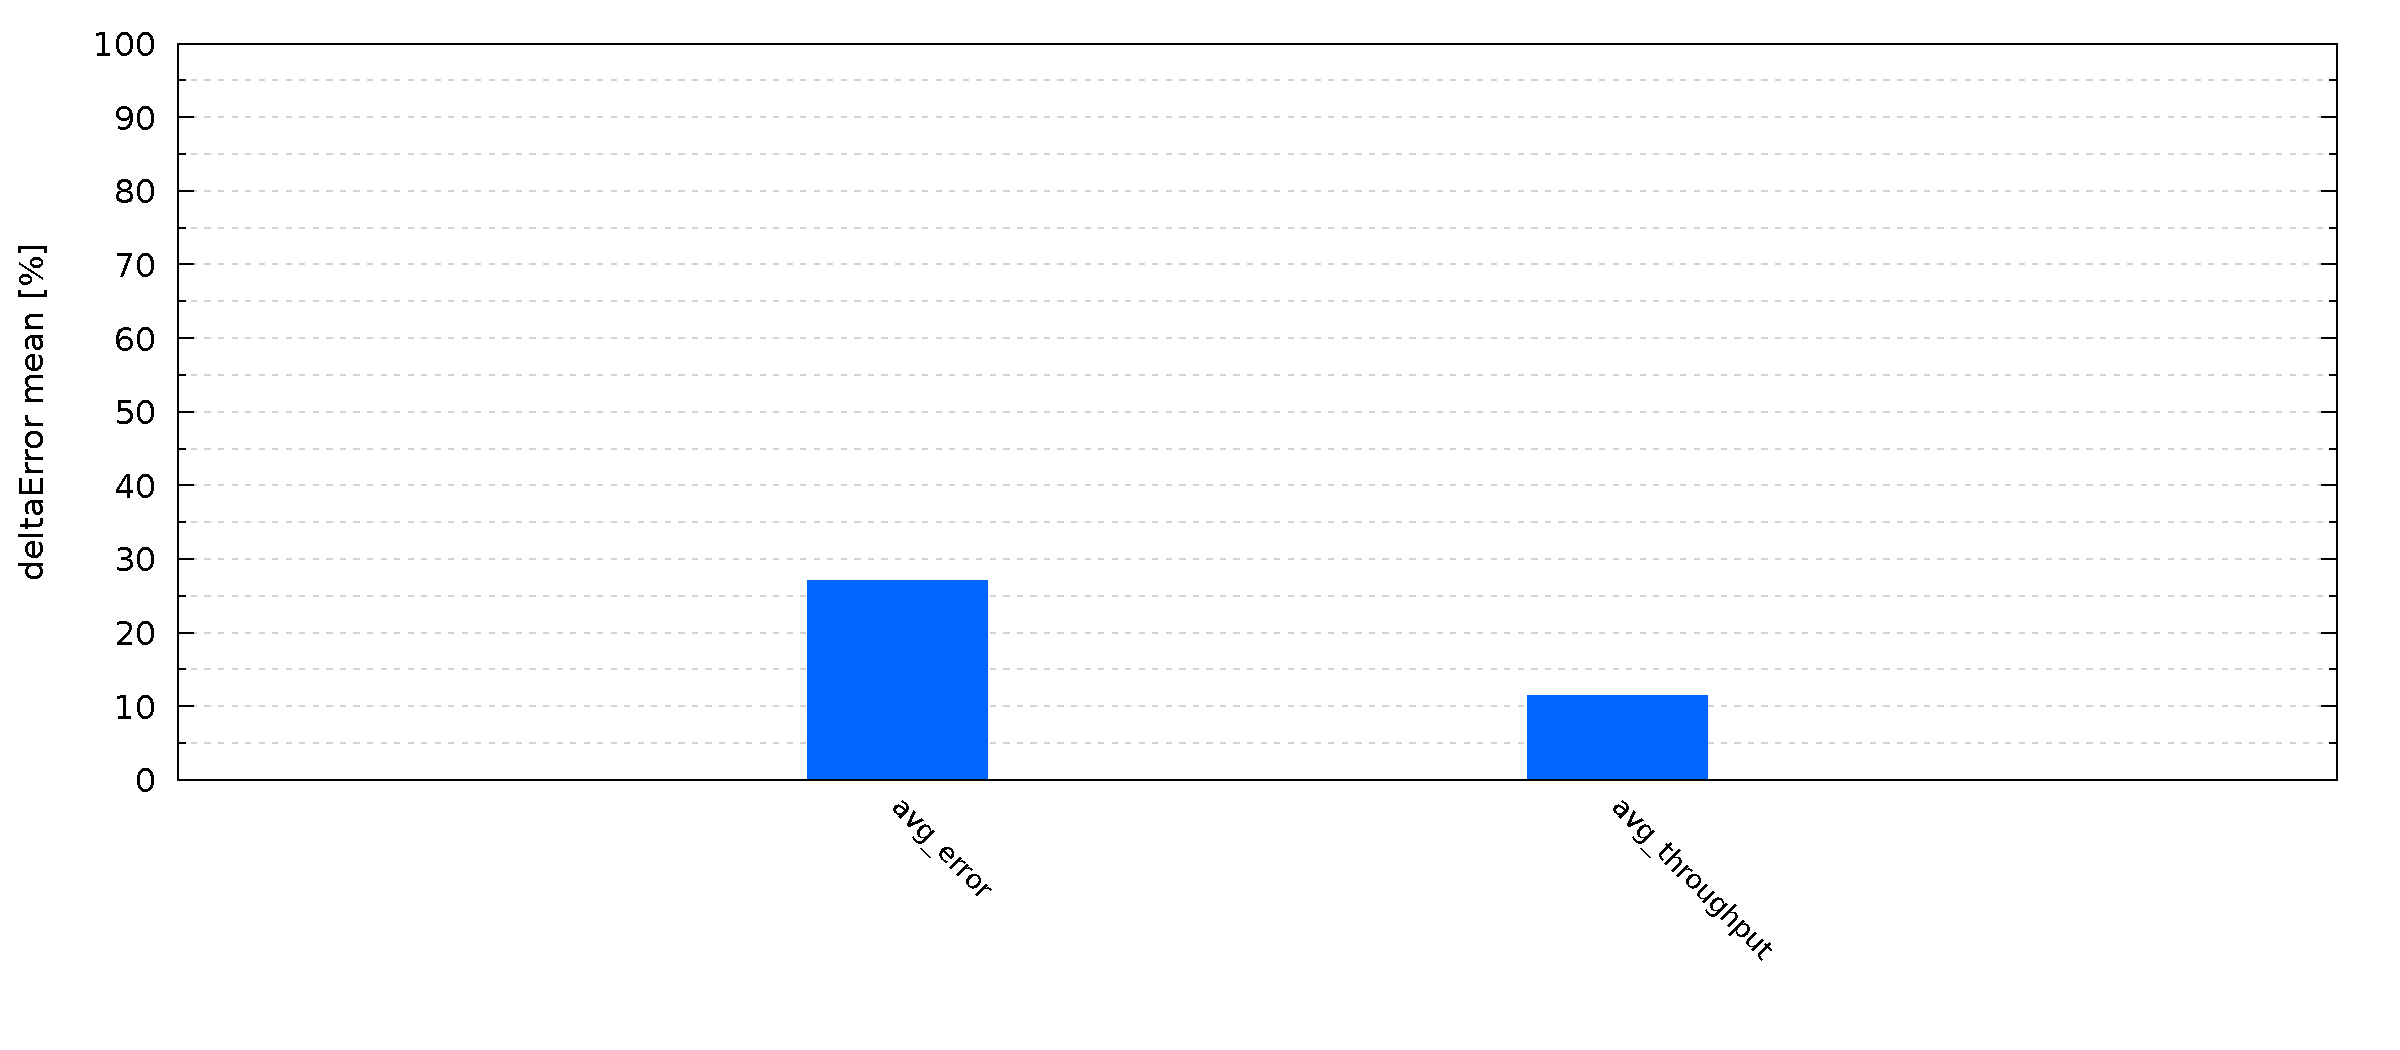
\includegraphics[width = \textwidth]{deltaErrorMeansSwaptions15Spark2}
    \caption{$deltaError$ mean values for both Swaptions metrics of interest}
    \label{fig::swaptions15spark2::means}
    
\end{figure}





We obtain an average $deltaError$ of around $11\%$ for $avg\_throughput$ and about $27\%$ for $avg\_error$, as it is shown in figure \ref{fig::swaptions15spark2::means}; from figure \ref{fig::swaptions15spark2::intervals} we can see that $70\%$ of $avg\_throughput$ predictions has a $deltaError$ below $15\%$, while this percentage increases to $30\%$ for $avg\_error$ metric.


\subsubsection{Execution times}

Regarding execution times, we compare analyzed run with a Full-Factorial, so exhaustive, execution in which we collect, for each configuration, 15 repetitions for each Operating Point, as shown in figure \ref{fig::sw::execT}:

\begin{figure}[h]

    \centering
    
    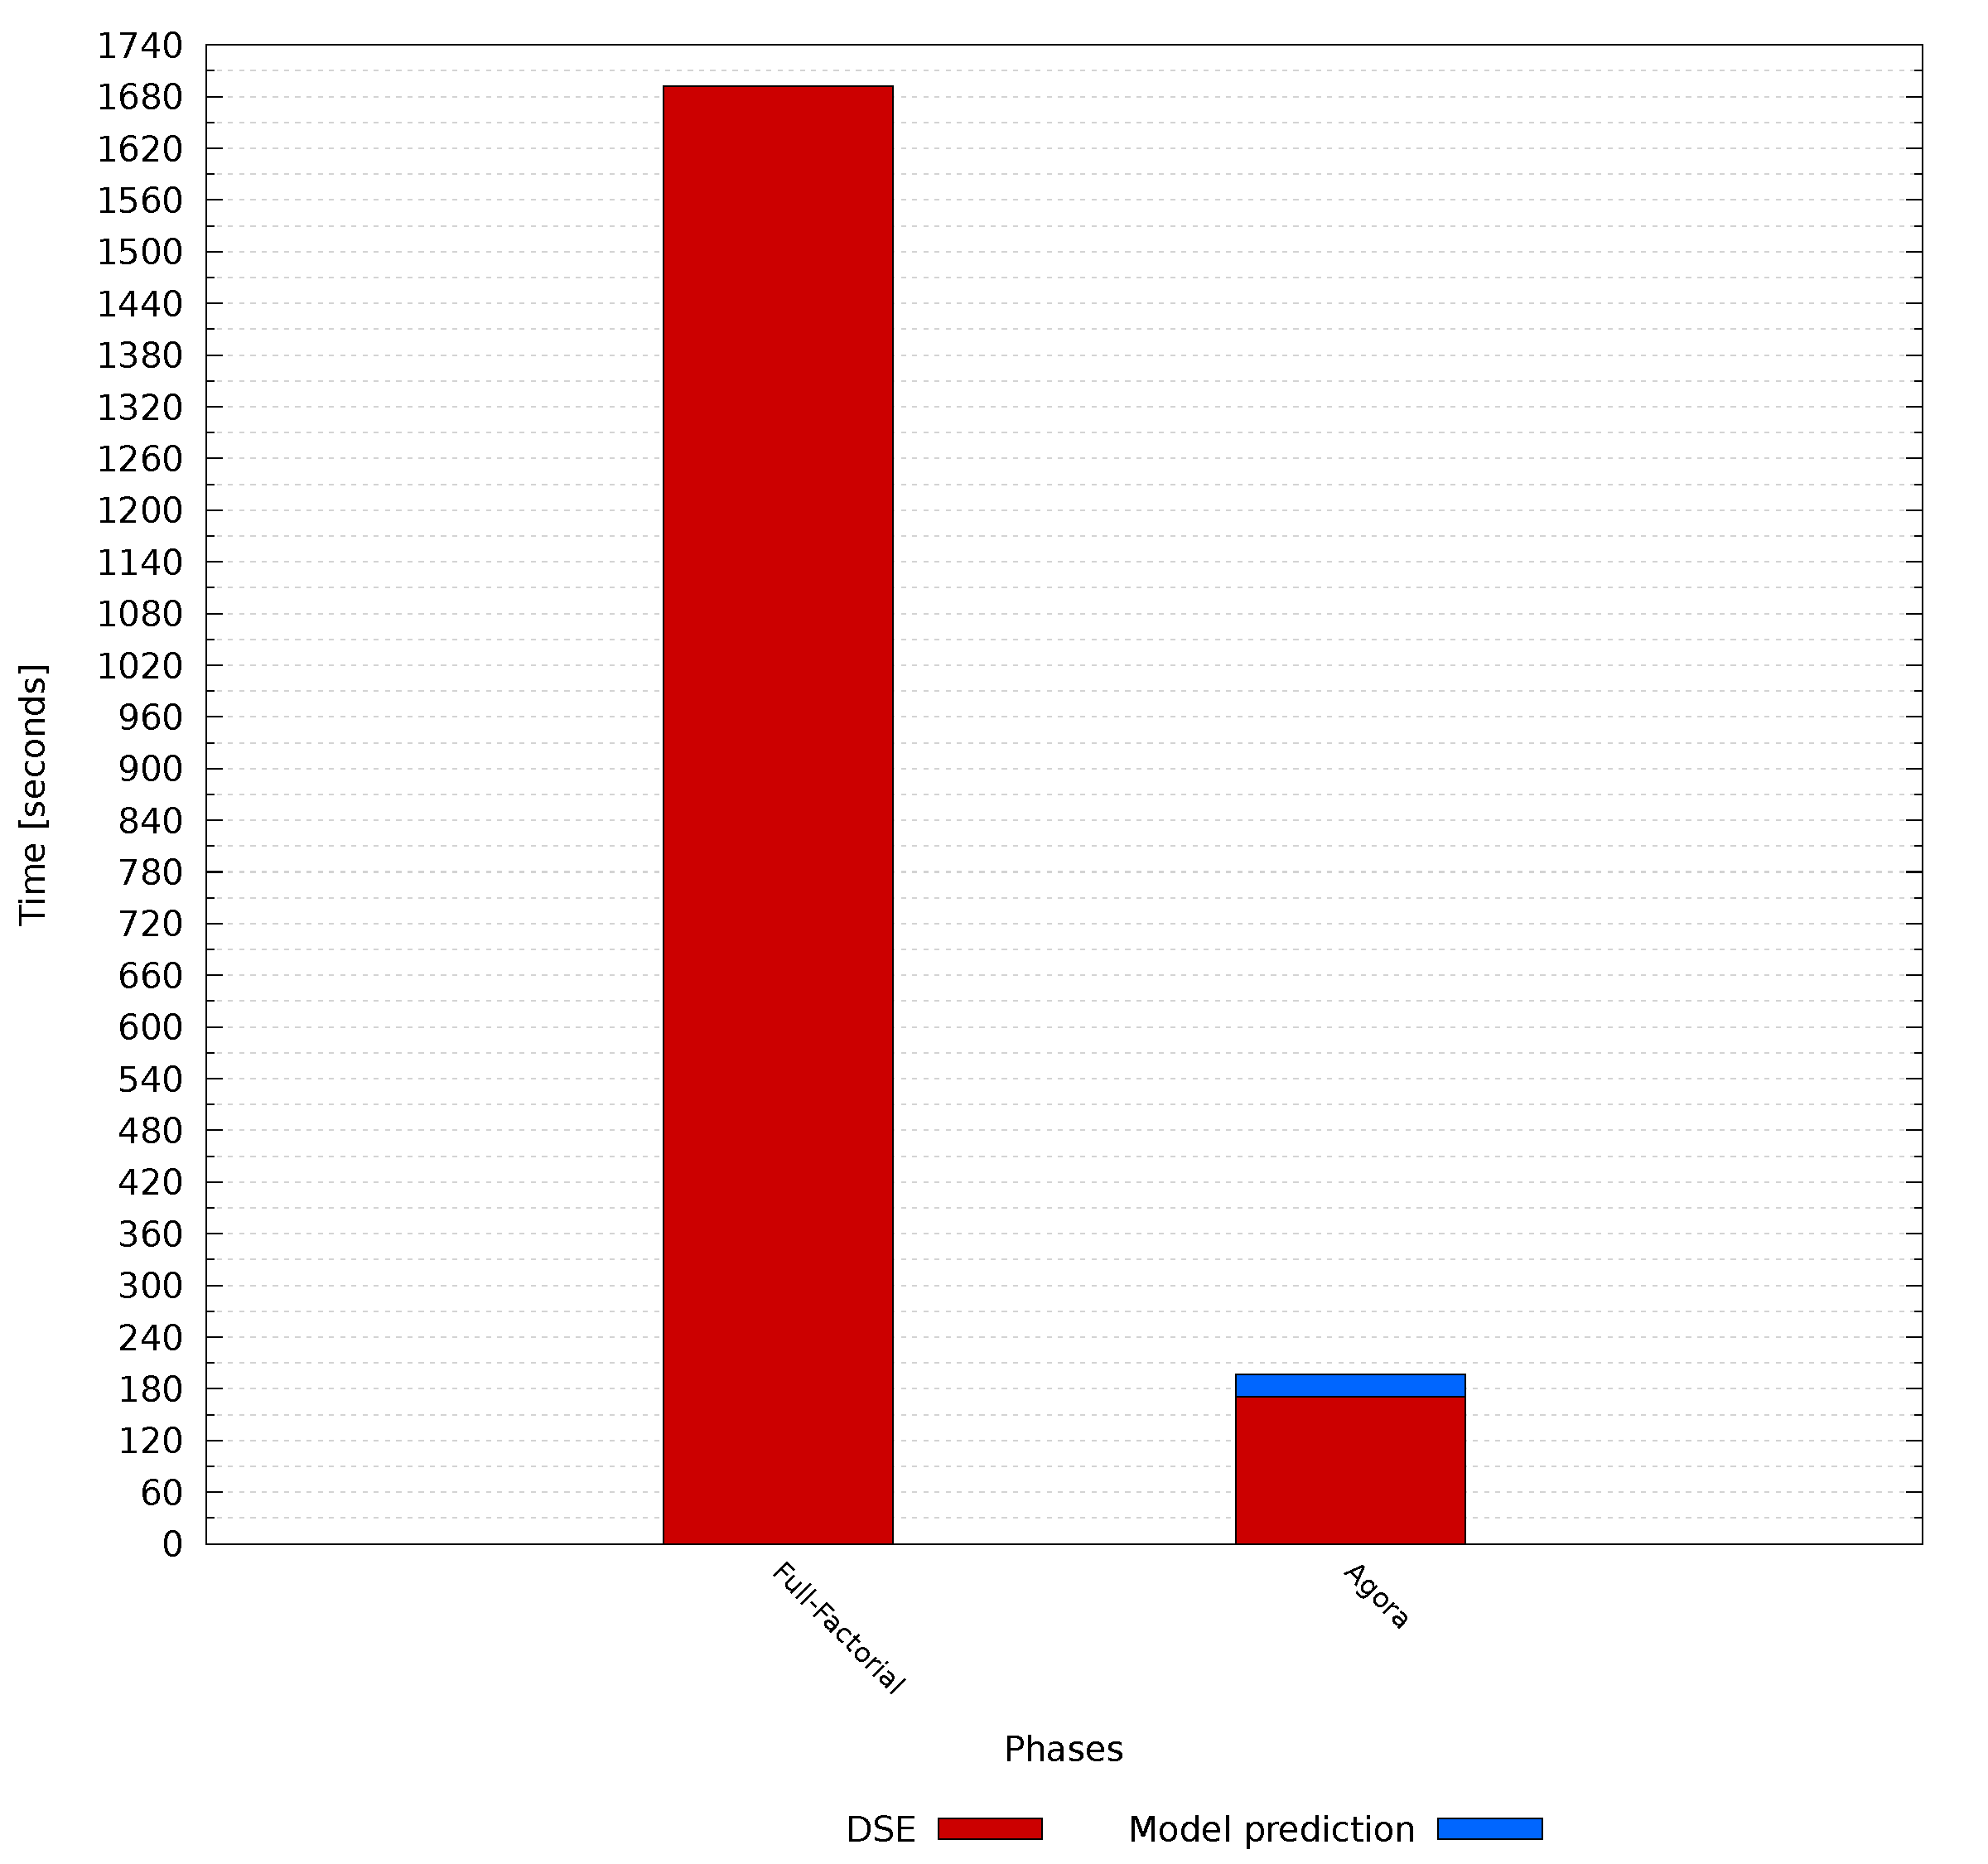
\includegraphics[width = \textwidth]{swaptions_exhaustive_tesiCris}
    
    \caption{Swaptions execution times}
    
    \label{fig::sw::execT}
    
\end{figure}

Exhaustive execution takes around 28 minutes to finish, while the analyzed one less than 3 and a half minutes, so approximately 8 times less; of course, as explained before, we do not obtain precise predictions for each metric value; nevertheless, \textit{Swaptions} can be executed with the assistance of Agorà plus mARGOt autotuner and, finally, prearranged objective functions are achieved, also because mARGOt is able to collect feedback information that corrects application model.


\subsubsection{Application behavior over time}

\begin{figure}[h]

    \centering
    
    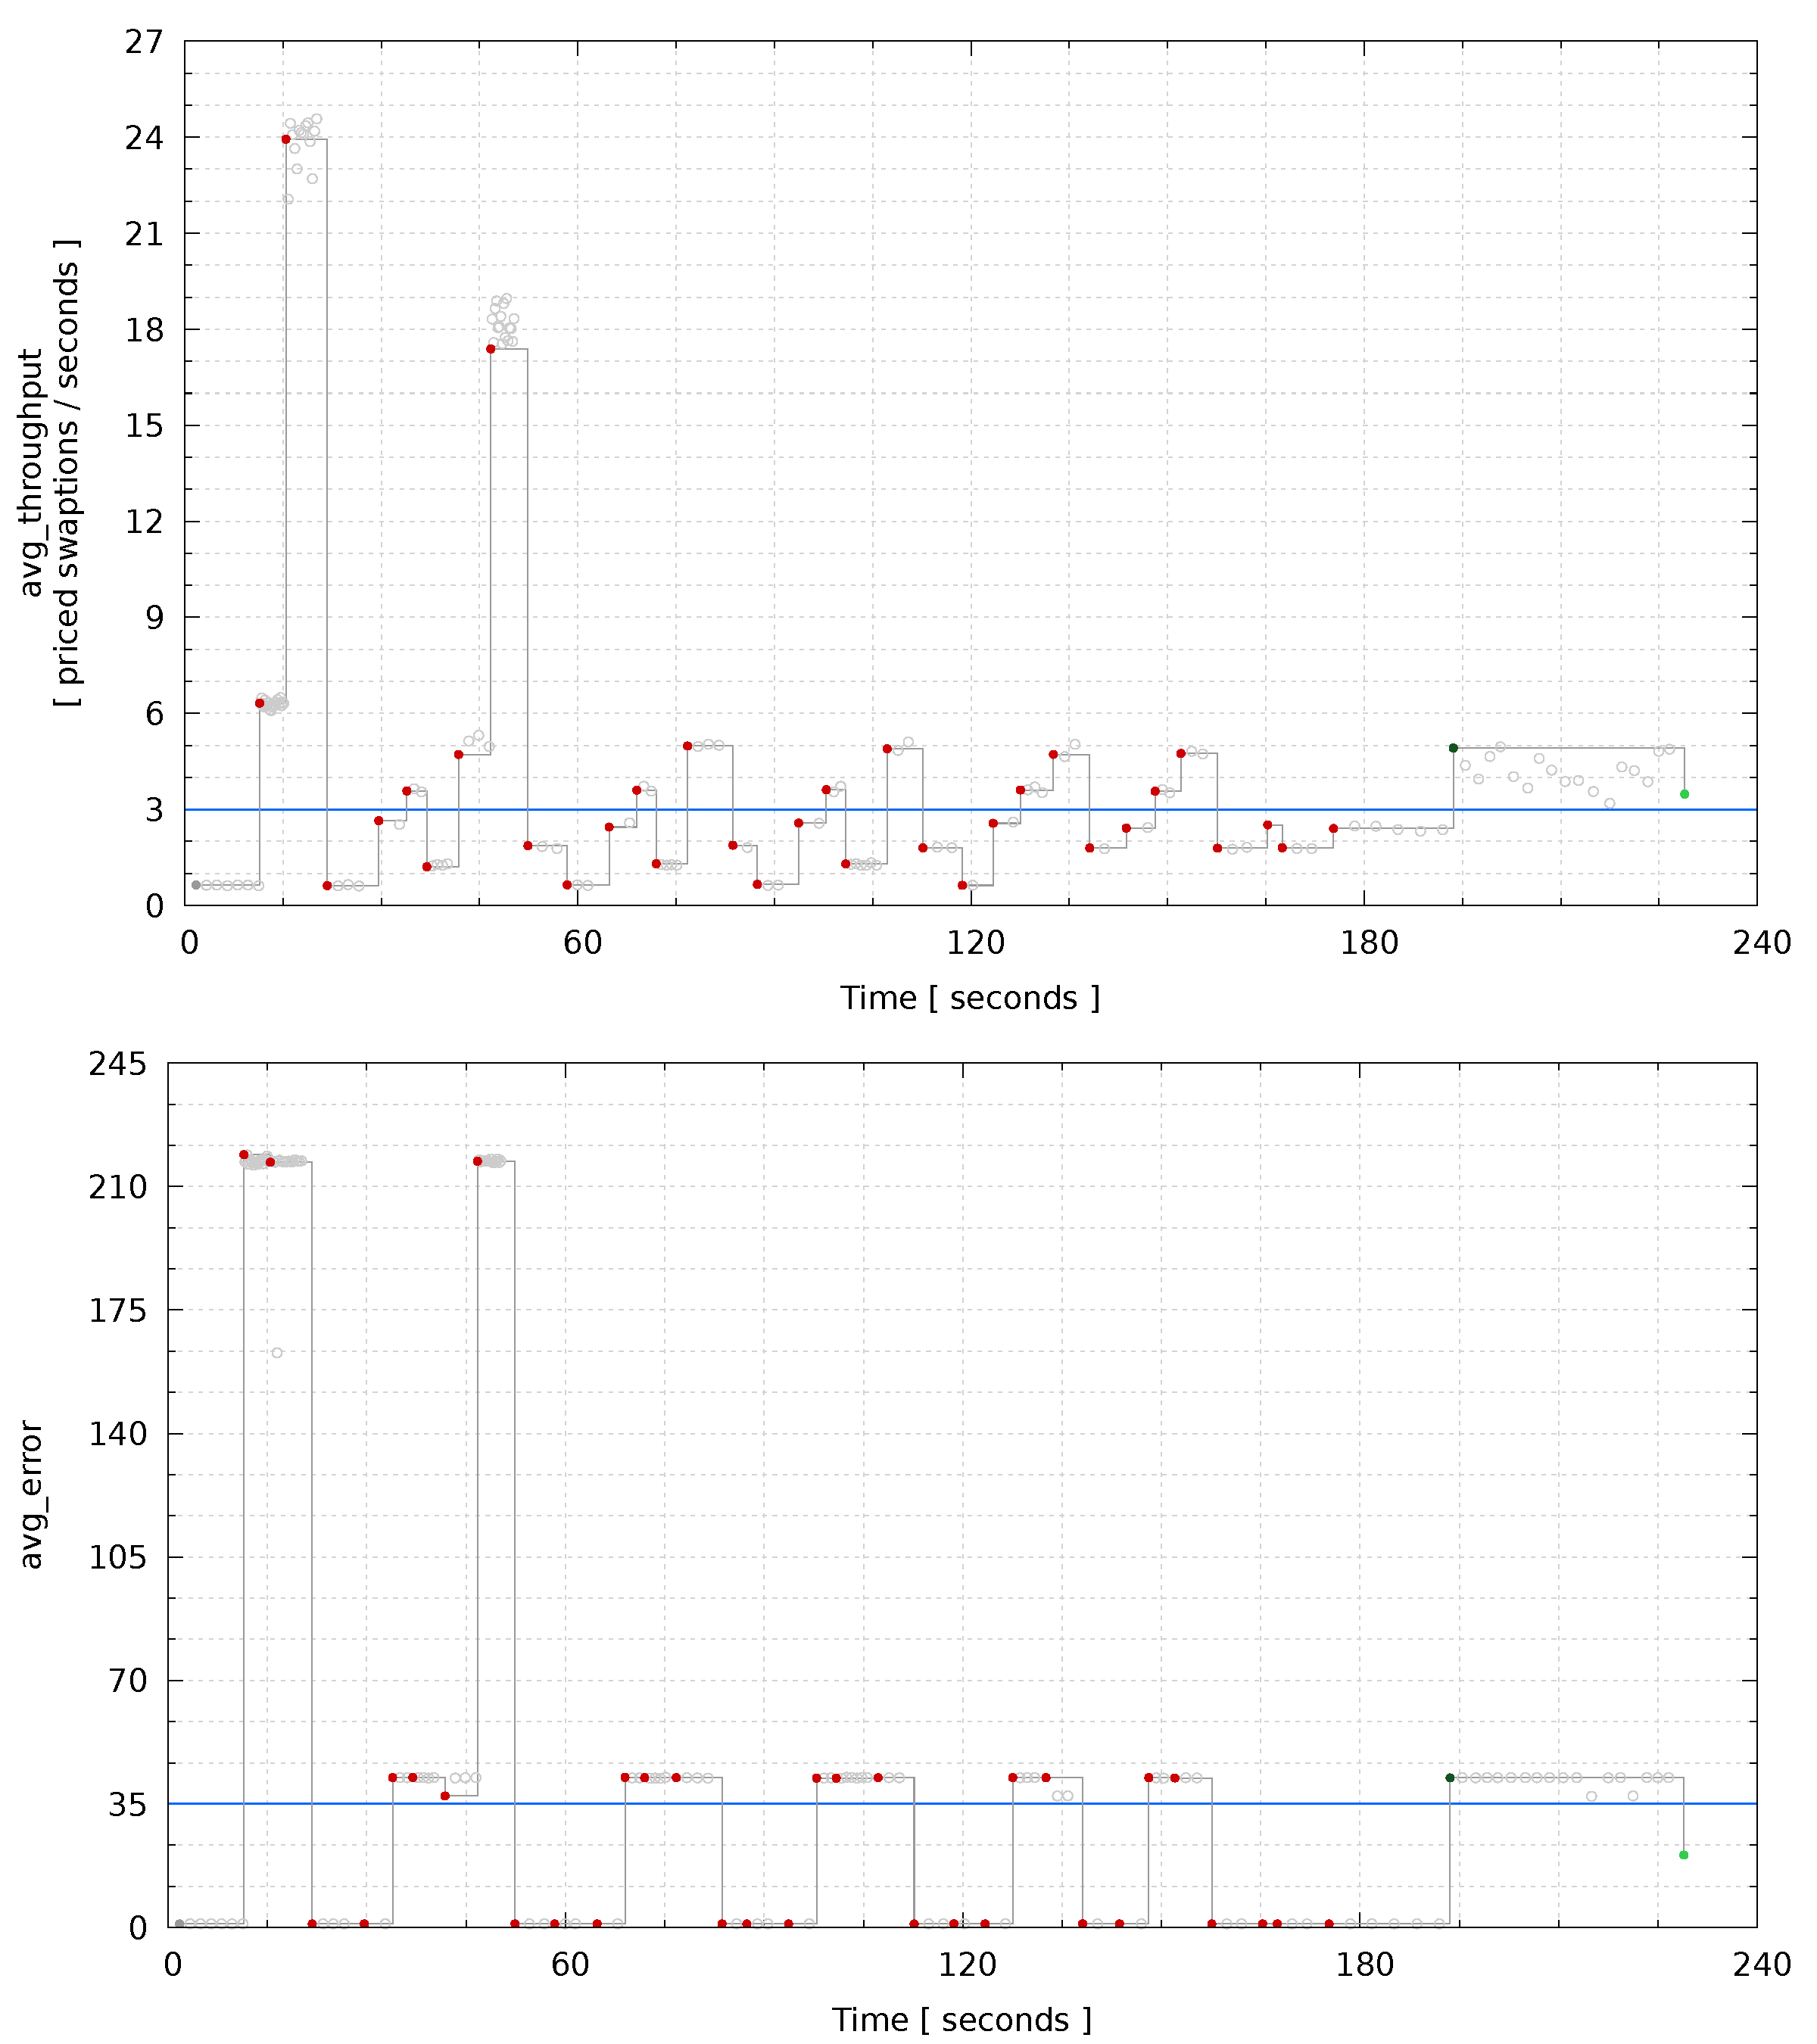
\includegraphics[width = \textwidth]{swaptionsBehavior}
    
    \caption{Swaptions metric values by varying time}
    
    \label{fig::sw::beh}
    
\end{figure}

Figure \ref{fig::sw::beh} shows application behavior during execution; we set, as objective functions, $avg\_\-throughput > 3$ and $avg\_\-error < 35$ (blue lines highlight boundaries of objective functions); during Design Space Exploration phase, application is executed with Design of Experiments configurations in order to collect training data (red couples of points); around 195 seconds, DSE phase finishes and application receives partial model (see \ref{DoEModelSend}); mARGOt sets up \textit{Swaptions} with best possible parameter values with respect to goals and requirements (dark green couple of points): during model prediction phase, $avg\_throughput$ is about 5 (so, great\-er than the minimum required value 3) and $avg\_error$ approximately 42 (higher than 35, so the corresponding objective function is not followed); Agorà sends complete model with predicted metric values for each application configuration: mARGOt changes current Operating Point (light green couple of points), obtaining an $avg\_throughput > 3$ and an $avg\_error < 35$, so both objective functions are achieved. 
